\documentclass[11pt,xcolor=table]{beamer}
\usetheme{CambridgeUS}
\usecolortheme{dolphin}

\usepackage[utf8]{inputenc}
\usepackage[L7x]{fontenc}
\usepackage[lithuanian]{babel}
\usepackage{lmodern} %be neveikia bold, italic etc


\usepackage{amsmath}
\usepackage{amsfonts}
\usepackage{amssymb}

\usepackage{graphicx}
\graphicspath{{./figures/}}

\usepackage{adjustbox}
\usepackage{bm}
\usepackage{subcaption}

\usepackage{multirow} % for multirow tables
\setbeamertemplate{caption}[numbered] % for numbering captions

\usepackage{forest}

\usepackage{listings}
\usepackage{color}
\usepackage{textcomp}
\definecolor{listinggray}{gray}{0.9}
\definecolor{lbcolor}{rgb}{0.9,0.9,0.9}
\lstset{
	backgroundcolor=\color{lbcolor},
	tabsize=4,
	rulecolor=,
	language=bash,
        basicstyle=\scriptsize,
        upquote=true,
        aboveskip={0.5\baselineskip},
        belowskip={0.5\baselineskip},
        columns=fixed,
        showstringspaces=false,
        extendedchars=false,
  breaklines=true,
  postbreak=\mbox{\textcolor{red}{$\hookrightarrow$}\space},
        frame=single,
        showtabs=false,
        showspaces=false,
        showstringspaces=false,
        identifierstyle=\ttfamily,
        keywordstyle=\color[rgb]{0,0,1},
        commentstyle=\color[rgb]{0.133,0.545,0.133},
        stringstyle=\color[rgb]{0.627,0.126,0.941},
                numbers=left,
        numbersep=5pt
}


\usepackage{tikz, pgfplots}
\usetikzlibrary{patterns,decorations.pathreplacing}


\author{Justas Mundeikis}
\title{Duomenų analizės įvadas}
\subtitle{1. Dalis}
%\setbeamercovered{transparent} 
%\setbeamertemplate{navigation symbols}{} 
%\logo{} 
%\institute{Vilniaus Universitetas, EVAF} 
%\date{} 
%\subject{} 


\setbeamerfont{subsection in toc}{size=\scriptsize}
%----------------------------------------------------------
\begin{document}
%----------------------------------------------------------

\begin{frame}
\titlepage
\end{frame}

%----------------------------------------------------------

\begin{frame}{1. Dalies turinys}
\tableofcontents
\end{frame}

%----------------------------------------------------------
\section{Įvadas į duomenų analizę}
%----------------------------------------------------------
%----------------------------------------------------------
\subsection{Duomenų analizės menas}
%----------------------------------------------------------

\begin{frame}{Duomenų analizės menas}
\begin{center}
\begin{figure}
\caption{To paties matymas kitaip}
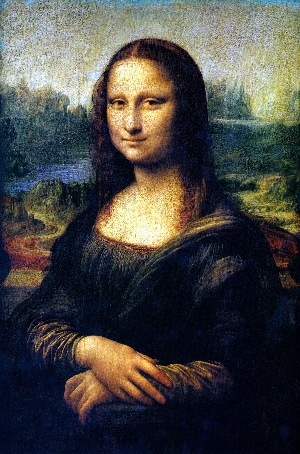
\includegraphics[width=.2\linewidth]{mona_lisa_1.jpg}\quad
\includegraphics[width=.2\linewidth]{mona_lisa_2.jpg}\quad 
\includegraphics[width=.2\linewidth]{mona_lisa_3.jpg}\quad

\includegraphics[width=.2\linewidth]{mona_lisa_4.jpg}\quad
\end{figure}
\end{center}
\end{frame}

%----------------------------------------------------------

\begin{frame}{Duomenų analizės menas}
\begin{figure}
\caption{Taip atrodo "duomenys"}
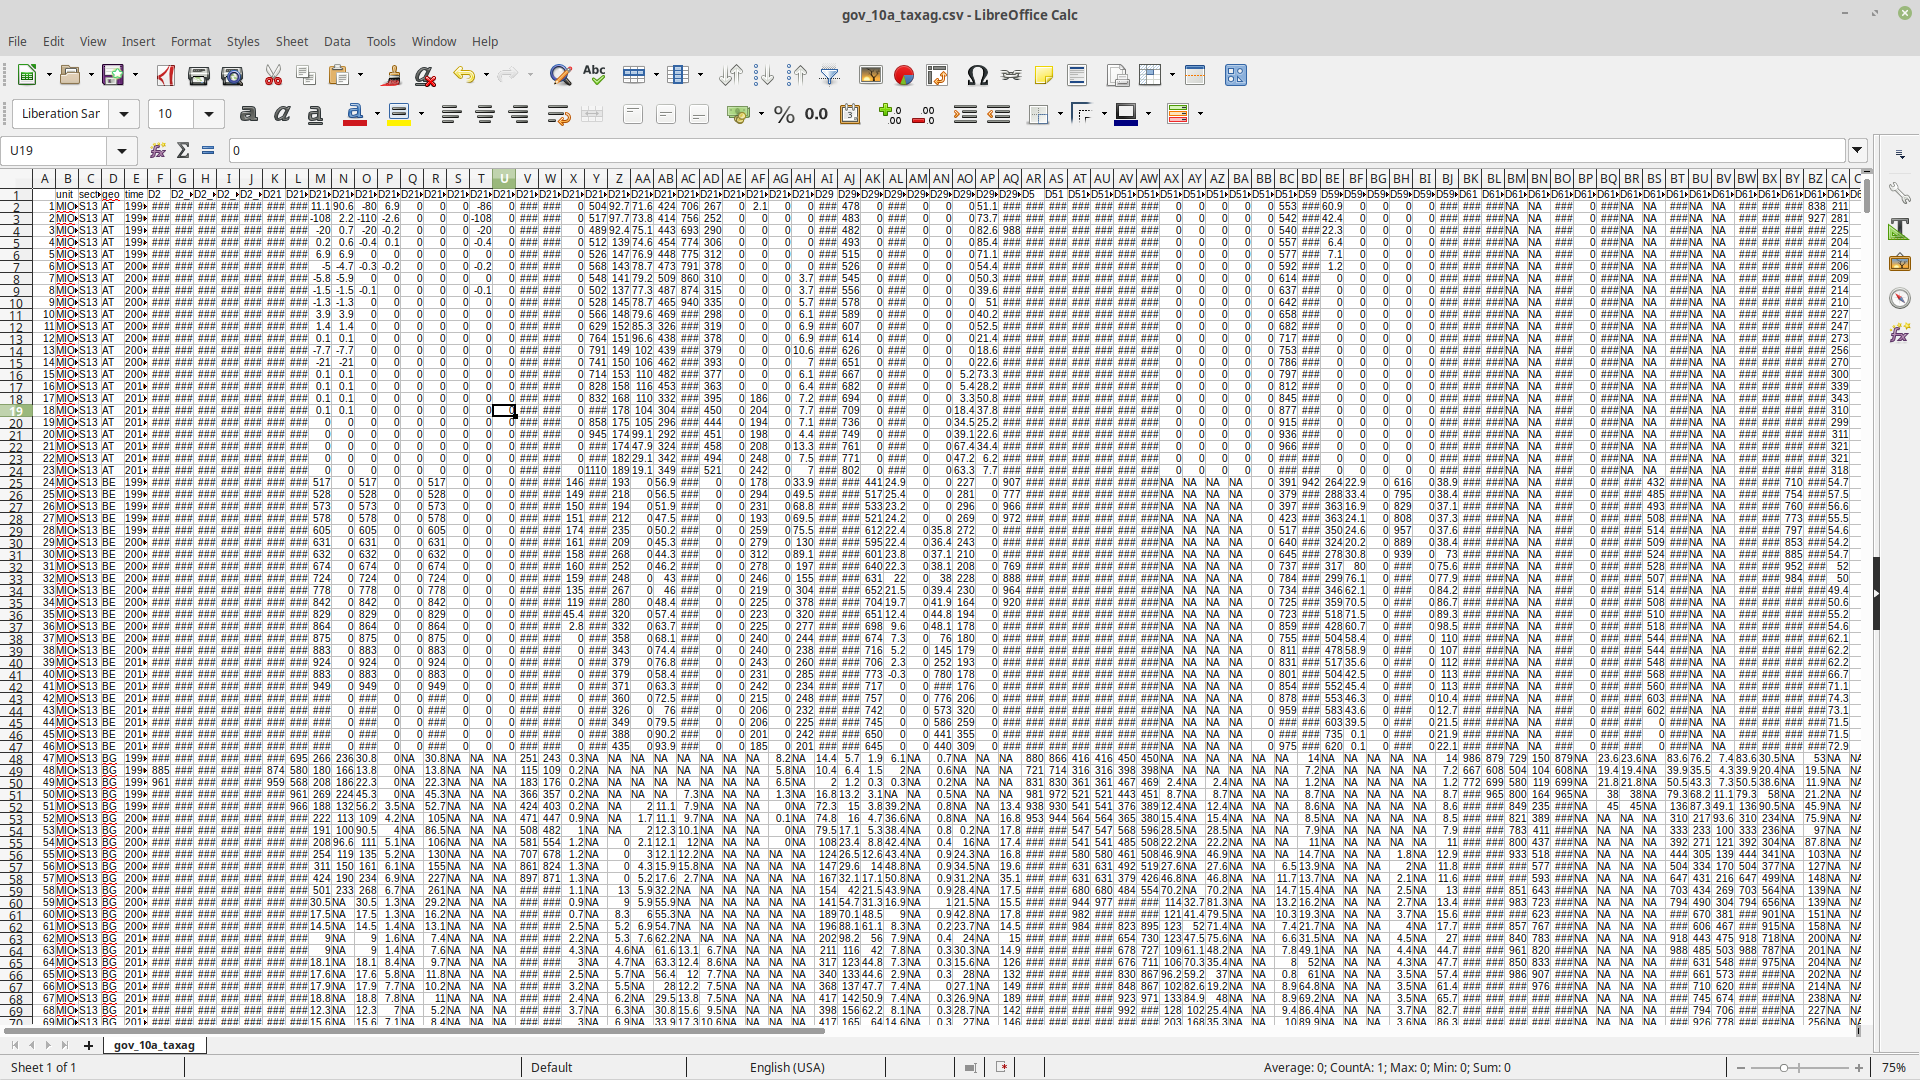
\includegraphics[scale=0.17]{raw_data.png}
\end{figure}
\end{frame}

%----------------------------------------------------------

\begin{frame}{Duomenų analizės menas}
\begin{figure}
\caption{Taip atrodo, ką galima padaryti su duomenimis}
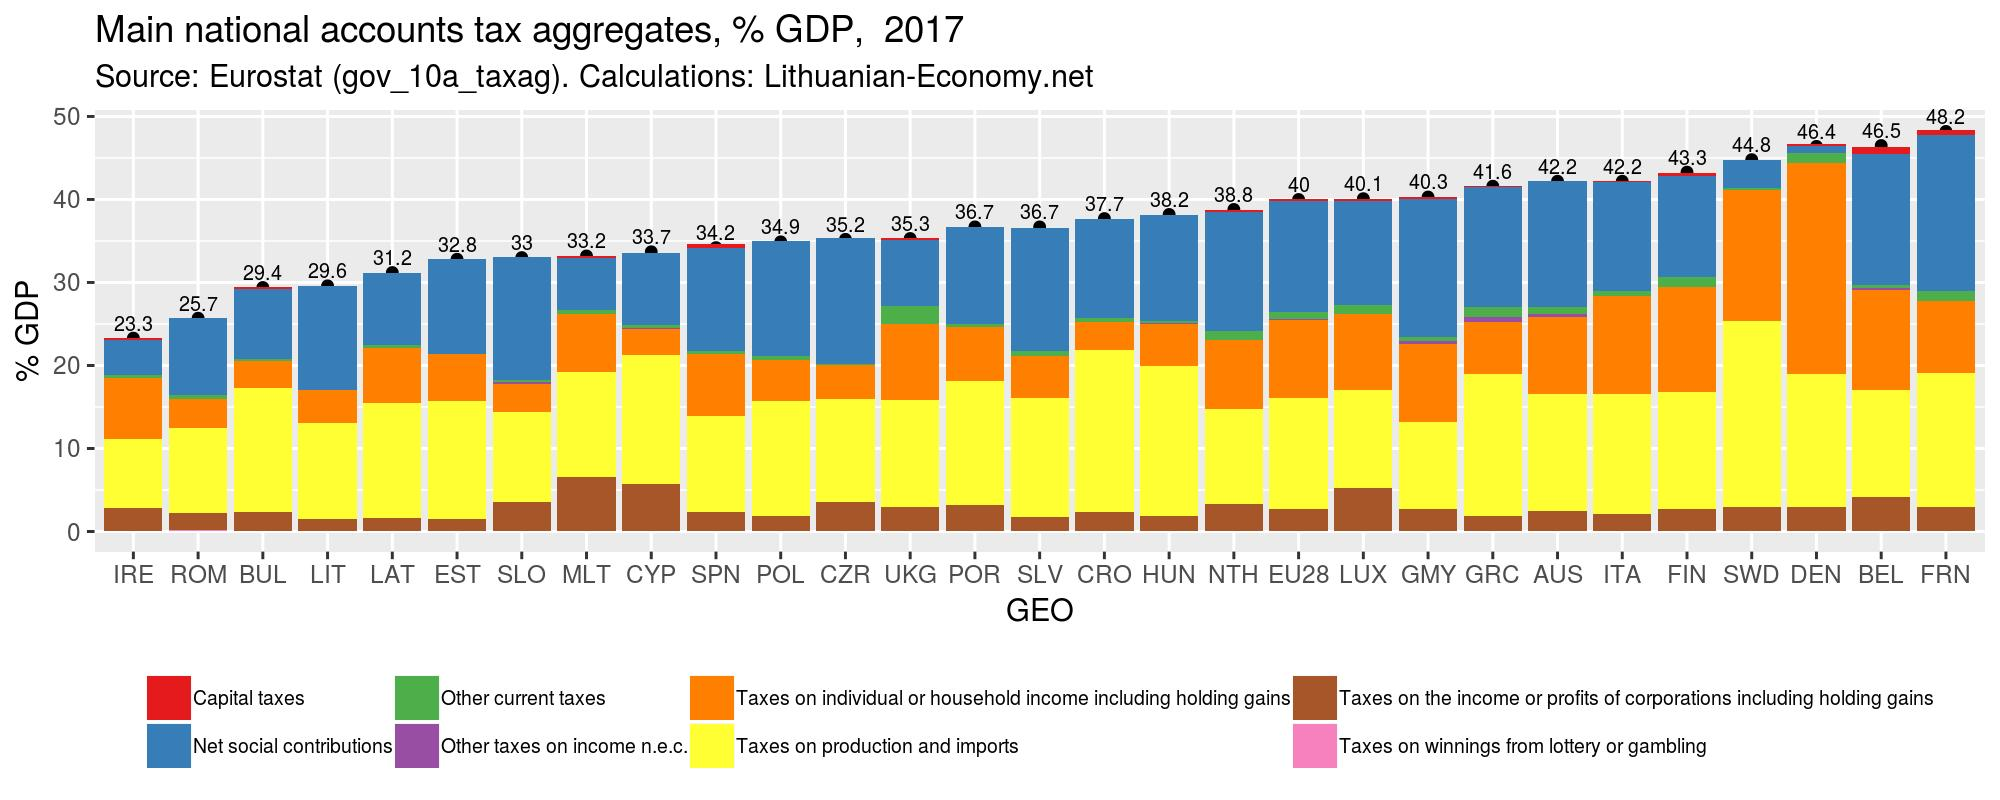
\includegraphics[scale=0.45]{Tax_GDP_2017_EU.jpeg}
\end{figure}
Trumpa diskusija: ar Lietuvos Tax/GDP (29.6 \%) yra gerai, ar blogai?
Gal verta perimti Airijos modelį?
\end{frame}


%----------------------------------------------------------

\begin{frame}{Duomenų analizės menas}
\begin{itemize}
\item \textit{"Science is knowledge which we understand so well that we can teach it to a computer; and if we don't fully understand something, it is an art to deal with it."}
\\Donald Knuth (1974) (\href{http://www.paulgraham.com/knuth.html}{\color{blue}{Knuth: Computer Programming as an Art}})
\item Neegzistuoja jokio formalaus aprašymo, kaip reikia atlikti "duomenų analizę"
\item Nors yra žinomi tam tikri įrankiai, statistiniai, ekonometriniai metodai, kuriais galima naudotis...
\item Kiekvieno "tyrėjo" (ekonomisto, duomenų analitiko, studento...) asmeninių pasirinkimų aibė nulemia atliekamos analizės kokybę bei naudą
\end{itemize}
\end{frame}



%----------------------------------------------------------
\subsection{Duomenų analizės epiciklai}
%----------------------------------------------------------

\begin{frame}{Mokslinio tyrimo žingsniai}
\begin{itemize}
\item {\color{red}{Labai daug skaityti}} (Savaitiniai skaitiniai: 3-6 straipsnius per savaitę, žinių (testo) dalis!)
\item {\color{blue}{Išvystyti klausimą / hipotezę}}
\item Nuspręsti kokia metodika bus taikoma
\item Parengti duomenų surinkimo procesą (tyrimo protokolas)
\item Surinkti duomenis
\item {\color{blue}{Atlikti tiriamąją statistiką}}
\item Atlikti aprašomąją statistiką
\item {\color{blue}{Modeliuoti, atlikti prognozes
\item Interpretuoti rezultatus
\item Aprašyti tyrimo eigą bei rezultatus}}
\end{itemize}
\end{frame}

%----------------------------------------------------------
\begin{frame}{Duomenų analizės žingsnių epiciklai}
% Please add the following required packages to your document preamble:
% \usepackage[normalem]{ulem}
% \useunder{\uline}{\ul}{}
\begin{table}[]
\caption{The Art of Data Science (Roger D. Peng \& Elizabeth Matsui)}
\label{my-label}
\scalebox{0.7}{
\begin{tabular}{|l|l|l|l|}
\hline
\textbf{Epycicles of analysis} & \textbf{Set expectations} & \textbf{Collect information} & \textbf{\begin{tabular}[c]{@{}l@{}}Revise\\ expectations\end{tabular}} \\ \hline
Question & \begin{tabular}[c]{@{}l@{}}Question is of interest\\ to audience\end{tabular} & \begin{tabular}[c]{@{}l@{}}Literature search\\ / Experts\end{tabular} & Sharpen question \\ \hline
EDA & \begin{tabular}[c]{@{}l@{}}Data are appropriate \\ for question\end{tabular} & \begin{tabular}[c]{@{}l@{}}Make exploratory \\ plots of data\end{tabular} & \begin{tabular}[c]{@{}l@{}}Refine question or \\ collect more data\end{tabular} \\ \hline
Formal modeling & \begin{tabular}[c]{@{}l@{}}Primary model \\ answers question\end{tabular} & \begin{tabular}[c]{@{}l@{}}Fit secondary models,\\ sensitivity analysis\end{tabular} & \begin{tabular}[c]{@{}l@{}}Revise formal model\\ to include \\ more predictors\end{tabular} \\ \hline
Interpretation & \begin{tabular}[c]{@{}l@{}}Interpretation of analyses\\ provides a specific \&\\ \\ meaningful answer to the\\ question\end{tabular} & \begin{tabular}[c]{@{}l@{}}Interpret totality of \\ analyses with focus \\ on effect sizes \& \\ uncertainty\end{tabular} & \begin{tabular}[c]{@{}l@{}}Revise EDA and / or\\ models to provide\\ specific \& \\ interpretable answer\end{tabular} \\ \hline
Communication & \begin{tabular}[c]{@{}l@{}}Process \& results of\\ analysis are understood, \\ complete \& meaningful\\ to audiance\end{tabular} & Seek feedback & \begin{tabular}[c]{@{}l@{}}Revise analyses or\\ approach to\\ presentation\end{tabular} \\ \hline
\end{tabular}
}
\end{table}
\end{frame}

%----------------------------------------------------------

\begin{frame}{Duomenų analizės žingsnių epiciklai}
\begin{figure}
\caption{The Art of Data Science (Roger D. Peng \& Elizabeth Matsui)}
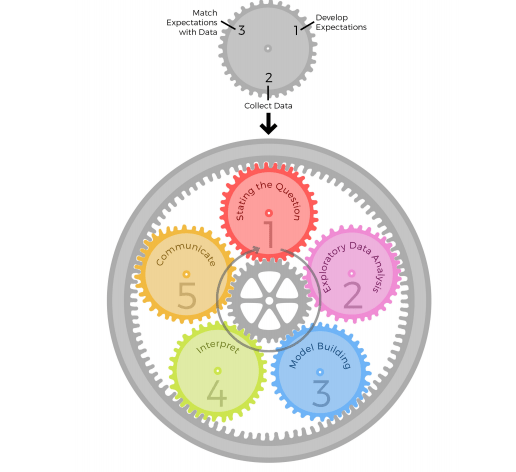
\includegraphics[scale=0.49]{Epicycles-of-Analysis.png}
\end{figure}

\end{frame}


%----------------------------------------------------------
\subsection{Duomenų analizės klausimai}
%----------------------------------------------------------

\begin{frame}{6 Klausimų tipai}
Remiantis R.Peng ir J.Leek (\href{www.sciencemag.org/content/347/6228/1314.short}{\color{blue}{Science 2015}}) egzistuoja 6 klausimų tipai:
\begin{itemize}
\item Aprašomieji
\item Tiriamieji
\item Inferenciniai
\item Progozuojamieji
\item Pražastinių ryšių
\item Mechanistiniai
\end{itemize}
\end{frame}
%----------------------------------------------------------
\begin{frame}{6 Klausimų tipai}
Aprašomieji klausimai:
\begin{itemize}
\item Kuriais siekiama gauti duomenų aprašymą, arba charakteristikų santraukas
\item Nedaromos jokios išvados ar prognozės, nes patys rezultatai yra išvados per se
\item Pvz., Moterų ir vyrų dalis tyrimo imtyje, vidutinis tiriamųjų amžius, vidutinė metinė infliacija, medianinės pajamos ir t.t.
\item \href{https://osp.stat.gov.lt/pagrindiniai-salies-rodikliai}{\color{blue}{LSD šalies rodikliai}}
\item \href{https://osp.stat.gov.lt/statistika-vizualiai}{\color{blue}{LSD statistika vizualiai}}
\end{itemize}
\end{frame}

%----------------------------------------------------------

\begin{frame}{6 Klausimų tipai}
Tiriamieji klausimai
\begin{itemize}
\item Klausimai, kuriais siekiama nustatyti sąsajas bei trendus
\item Padeda rasti kelią kuriuo galima judėti tyrime pirmyn, pvz., generuoti hipotezes
\item Dažniausiai tokių klausimų atsakymui braižomi grafikai, padedantys surpasti duomenis
\item Tačiau "Correlation does not imply causation" (žr sekanti skaidrė!!!)
\end{itemize}
\end{frame}

%----------------------------------------------------------
\begin{frame}{6 Klausimų tipai}
\begin{figure}
\caption{Šokolado vartojimas ir Nobelio prizai (\href{https://www.nejm.org/doi/full/10.1056/NEJMon1211064}{\color{blue}{Franz H. Messerli, M.D., 2012}})}
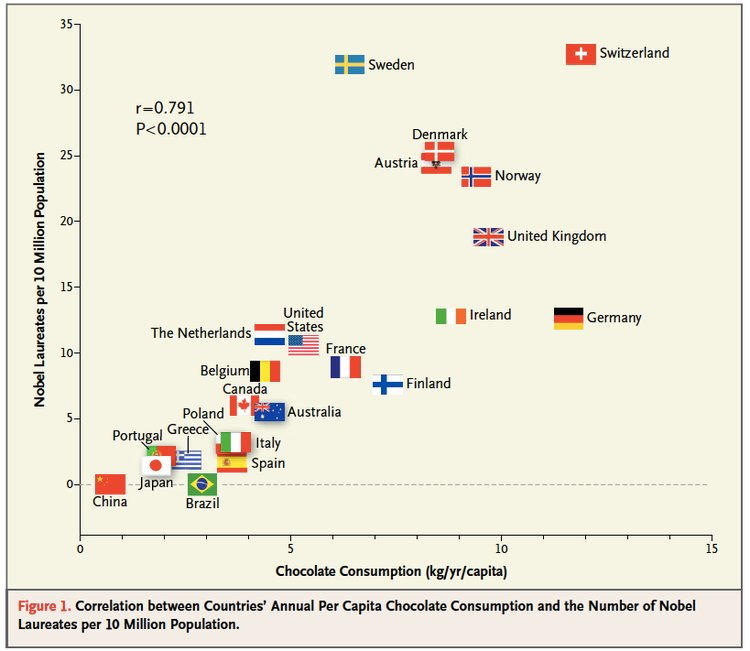
\includegraphics[scale=0.28]{schockolade_nobel.jpg}
\end{figure}
\end{frame}

%----------------------------------------------------------

\begin{frame}{6 Klausimų tipai}
Inferenciniai klausimai:
\begin{itemize}
\item Klausimai, kuriais siekiama atsakyti klausimus apie bendrą populiaciją, tiriant tik imtį
\item Pvz., Ekonomikos kurso 1 gr. baigiamasis pažymys 8. Ar visas 1 kursas gavo 8?
\item Taikant inferencinę analizę siekiama nustatyti dominantį kiekį bei su prognoze susijusią paklaidą
\end{itemize}
\end{frame}
%----------------------------------------------------------

\begin{frame}{6 Klausimų tipai}
Prognozuojamieji klausimai
\begin{itemize}
\item Klausimai, kuriais siekiama "atspėti" ateitį 
\item Naudojant turimą informaciją apie tam tikrus objektus prognozuoti reikšmes kitiems objektams
\item Svarbu: Jeigu X prognozuoja Y nereiškia, kad X iššaukia Y
\item Prognozavimo taiklumas priklauso nuo teisingo matuojamų kintamųjų pasirinkimo
\item Kuo daugiau duomenų ir kuo paprastesnis modelis!
\item \href{https://fivethirtyeight.com/}{\color{blue}{https://fivethirtyeight.com/}}
\item \href{https://www.amazon.com/Lenovo-ThinkPad-Performance-Business-fingerprint/dp/B077GP6G9M/ref=sr_1_fkmr1_1?keywords=ibm+thinkpad+t460&qid=1549818100&s=gateway&sr=8-1-fkmr1}{\color{blue}{AMAZON IBM E570}}
\end{itemize}
\end{frame}
%----------------------------------------------------------
\begin{frame}{6 Klausimų tipai}
Priežastinių ryšių klausimai:

\begin{itemize}
\item Klausimai, norint sužinoti, ar pakeitus vieną faktorių, kinta kitas faktorius
\item \href{http://psyking.net/HTMLobj-4363/Effects_of_Sleep_Deprivation-Schumacher_and_Sipes-Final.pdf}{\color{blue}{How  does  a  lack  of  sleep  impact  memory,  problem  solvingand  critical  thinking  skills  amongstcollege students?}}
\item Reikalingos randomizuotos studijos
\item Ekspertimentų galimybė ekonomikos šakoje ribota
\item Yra būdų kaip tai apeiti (ekonometrika magistre / PhD)
\item Dažniausiai gaunami vidutiniai efektai
\item Siekiama atsakyti "ar" bet ne "kaip"
\end{itemize}
\end{frame}
%----------------------------------------------------------
\begin{frame}{6 Klausimų tipai}
Mechanistiniai klausimai
\begin{itemize}
\item Klausimai, kuriais siekiama nustatyti "kaip"
\item Kaip ir kokie būtent pokyčiai vieno kintamojo keičia daro įtaką kitiems kintamiesiems (fizikos/inžinerijos sritis)
\end{itemize}
\end{frame}

%----------------------------------------------------------

\begin{frame}{6 Klausimų tipai}
\begin{itemize}
\item Svarbu suprasti, jog pvz., iškėlus prognozuojamąjį klausimą, tyrimo eigoje   bus atsakyti ir į aprašomuosius, tiriamuosius, inferencinius klausimus 
\end{itemize}
\end{frame}

%----------------------------------------------------------
\begin{frame}{Koks yra geras klausimas?}
Geras klausimas pasižymi šiomis savybėmis:
\begin{enumerate}
\item Klausimas turi būti įdomus tikslinei auditorijai
\item Klausimas dar neturi būti atsakytas
\item Klausimas turi būti logiškas / prasmingas (pagrįstas teorija)
\item Klausimas turi būti atsakomas (netinka: "Kokia yra gyvenimo prasmė?/ Ar egzistuoja dievas?"), kitaip tariant, turi egzistuoti duomenys ir metodikos, kurių pagalba būtų galima atsakyti į klausimą
\item Klausimas turi būti labai konkretus
\begin{itemize}
\item Blogas klausimas: ar sveika mityba skatina ilgesnį gyvenimą
\item Geras klausimas: ar 250gr daržovių kasdien suaugusiam asmeniui padidina tikėtiną gyvenimo trukmę 10 metų?
\item Blogas klausimas: kas ekonomikos nuosmukio laikotarpiu nukenčia labiausiai
\item Geras klausimas: Kurioms iš soc grupių: bedarbiai, pensininkai, daugiavaikės šeimos per ekonominę 2008-2009 krizę labiausiai padidėjo rizika patirti santykinį skurdą 
\end{itemize}
\end{enumerate}
\end{frame}




%----------------------------------------------------------
\subsection{Duomenys, matavimo skalės}
%----------------------------------------------------------

\begin{frame}{Duomenys, matavimo skalės}
\begin{itemize}
\item Duomenys yra faktai arba skaičiai, kurie yra renkami, analizuojami bei apibendrinami pristatymo ar interpretavimo tikslais
\item Duomenys surinkti tam tikro tyrimo metu vadinami duomenų set'u arba duomenų masyvu
\item \textbf{Elementai} - subjektai, apie kurios renkami duomenys
\item \textbf{Kintamasis} - elemento charakteristika
\item Tyrimo metu surinkti \textbf{matavimai} apie visus dominančius elementus ir jų kintamuosius ir yra duomenys / duomenų set'as
\item Duomenų set'as vieno elemento vadinamas \textbf{obzervacija}
\end{itemize}
\end{frame}

%----------------------------------------------------------

\begin{frame}{Duomenys, matavimo skalės}
Kintamųjų tipas apibrėžia informacijos kiekį slypinti duomenyse, bet kartu ir apriboja galimus taikyti statistinius metodus jų analizei.
\begin{itemize}
\item \textbf{Kategoriniai} kintamieji:
\begin{itemize}
\item \textbf{Nominalūs} kintamieji: Lytis, Spalva
\\ Galima tik suskaičiuoti vienetus
\item \textbf{Ranginiai} kintamieji: Dydžiai S,M,L; Kredito reitingai F - AAA 
\\ Juos galima prasmingai suranguoti!
\end{itemize}
\item \textbf{Kiekybiniai} kintamieji:
\begin{itemize}
\item \textbf{Intervaliniai} kintamieji: pažymiai (neturi 0)
\\ +,-, yra prasmingi, bet daugyba, dalyba nėra prasmingi
\item \textbf{Santykiniai} kintamieji: svoris, ūgis, atstumas  (turi 0)
\\ +,-, daugyba, dalyba yra prasmingi
\end{itemize}
\end{itemize}
\end{frame}

%----------------------------------------------------------

\begin{frame}{Duomenys, matavimo skalės}
\begin{itemize}
\item 'Tarpsekciniai' duomenys (angl.: cross-sectional data): vienu ar panašiu metu užfiksuoti skirtingų elementų matavimai: pvz Europos šalių 2018m. BVP €
\item Laiko eilučių duomenys (angl.: Time series data): Matavimai surinkti per du ar daugiau laikotarpių vienam elementui
\item 'Tarpsekcinės' laiko eilutės (n elementų, t laikotarpiį, taigi $n \times t $ matavimų)
\end{itemize}
\end{frame}

%----------------------------------------------------------
\begin{frame}{Big Data}
\begin{itemize}
\item Lietuvoje dauguma įmonių nelabai supranta ką reiškia "big-data"
\item Big-data be AI perteklinis duomenų kaupimas
\item Problema su AI - niekas nesupranta AI
\item Tačiau su laiku AI keis ir ekonomikos mokslą:
\item \href{https://www.aeaweb.org/webcasts/2019/aea-afa-joint-luncheon-impact-of-machine-learning}{\color{blue}{Video: AEA AFA Joint Luncheon - The Impact of Machine Learning on Econometrics and Economics}}
\item John Tukey: "The data may not contain the answer. The combination of some data and an aching desire for an answer does not ensure that a reasonable answer can be extracted from a given body of data" 
\end{itemize}
\end{frame}

%----------------------------------------------------------

\begin{frame}{Apibendrinant:}
\begin{itemize}
\item Svarbiausias duomenų analizės / tyrimo aspektas - klausimas!
\item Antras pagal svarbumą - duomenys
\item Dažnai duomenys apribos arba išlaisvins Jus, 
\\bet tik duomenys be klausimo, neišgelbės :D
\end{itemize}
\end{frame}


%----------------------------------------------------------
\section{Command line interface}
%----------------------------------------------------------

\begin{frame}
\center

\includegraphics[scale=0.5]{cat_pc.jpeg}
\end{frame}

%----------------------------------------------------------
\subsection{Intro}
%----------------------------------------------------------

\begin{frame}{Command Line interface (CLI)}
Kiekviena operacinė sistema turi CLI:
\begin{itemize}
\item Windows: Git Bash (), CMD
\item Mac/ Linux: Terminal'as
\end{itemize}
Su CLI galima:
\begin{itemize}
\item Naviguoti tarp aplankų (folder'ių)
\item Kurti, keisti, naikinti: failus, aplankus, programas
\item Startuoti programas
\end{itemize}
\end{frame}

%----------------------------------------------------------
\begin{frame}{Intarpas GIT Bash instaliavimas}
\begin{itemize}
\item Nors darbiniai kompiuteriai turi instaliuotą Git Bash, tiems kas neturi:
\item \href{https://git-scm.com/}{\textcolor{blue}{https://git-scm.com/}}
\item Windows 32/64, Linux žr. komandą
\item Perimti teikiamus standartinius siūlymus, nebent antrame Setup lange pasirinkti, jog Git Bash rodytų ir "Addditional icons: On the desktop"
\item Startuojam Git Bash
\item Nuspaudus dešinį pelės mygtuką atsidaro meniu, einame ant \textit{Options..}
\begin{itemize}
\item Looks: pasirenkame Curser - Block (bent jau pradžiai, vėliau pasikeikite į \textit{line})
\item Keys: Ctrl+Shift+letter shortcuts pastarasis apsirinkimas leidžia daryti  naudoti Crtl+C, Crtl+V tačiau reikia kartu nuspausti ir Shift!
\end{itemize} 
\end{itemize}
\end{frame}
%----------------------------------------------------------
\begin{frame}{Direktorijos}
\begin{itemize}
\item \textit{Directory} yra tiesiog kitas pavadinimas žodžiui aplankas
\item Direktorijos kompiuteryje organizuotos kaip medžio šakos
\item CLI padeda naviguoti tarp šių direktorijų
\item "/" yra \textit{root directory} Linux, 
\item Windows \textit{root directory} yra C:
\item \textit{Root directory} talpina visas kitas direktorijas
\end{itemize}
\center
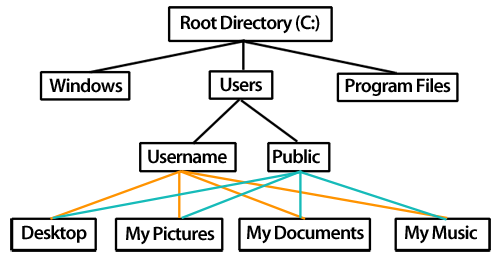
\includegraphics[scale=1.5]{diagram_directory_win.png}
\end{frame}

%----------------------------------------------------------
\subsection{Direktorijos}
%----------------------------------------------------------

\begin{frame}[fragile]{Direktorijos}
\begin{itemize}
\item Startavus matosi daug maž toks tekstas (priklausomai nuo kompiuterio jis gali skirtis!)

\begin{lstlisting}
USER@PC MINGW64 ~
$ 
\end{lstlisting}

\item \$ ženklas (angl.: promt) reiškia: "gali rašyti komandą"
\item Tipinis įrašas susideda iš: "command flag argument"
\item Komandos pvz: komanda liepianti atspausdinti kurioje direktorijoje esama: \colorbox{listinggray}{\lstinline|pwd|}

\begin{lstlisting}
USER@PC MINGW64 ~
$ pwd
/c/Users/USER
\end{lstlisting}

\end{itemize}
\end{frame}
%----------------------------------------------------------

\begin{frame}[fragile]{Direktorijos}
Universiteto kompiuteriuose pwd atsako:
\\/c/Users/studentas

\begin{figure}
\caption{Kur mes esame direktorijų medyje}

\end{figure}
\end{frame}


%----------------------------------------------------------
\subsection{CLI komandos}
%----------------------------------------------------------
\begin{frame}[fragile]{CLI komandos}
\begin{itemize}
\item Komanda gali būti iššaukiama su tam tikra programa
\item \colorbox{listinggray}{\lstinline|git init|} {\color{red}{šitos komandos dabar nenaudot!}}
\item \colorbox{listinggray}{\lstinline|python get-pip.py|}{\color{red}{šitos komandos dabar nenaudot!}}
\item flag: tam tikri nustatymai, galimi priklausomai nuo komandos ir visada su "-"
\item argument - kiti nustatymai, pakeitimai ar panašūs dalykai
\item \colorbox{listinggray}{\lstinline|git commit -m "this is the initial commit"|} {\color{red}{šitos komandos dabar nenaudot!}}
\item jeigu flag yra žodis , tada naudojami du brūkšniai -\/- 
\item \colorbox{listinggray}{\lstinline|git reset --hard HASH|} {\color{red}{šitos komandos dabar nenaudot!}}

\end{itemize}
\end{frame}

%----------------------------------------------------------

\begin{frame}[fragile]{CLI komandos}
\begin{figure}
\caption{komanda}
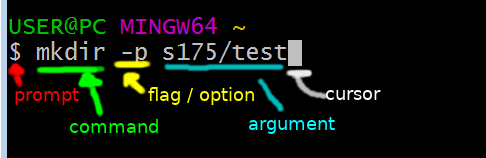
\includegraphics[scale=0.7]{command.png}
\end{figure}
\end{frame}

%----------------------------------------------------------
\begin{frame}[fragile]{CLI komandos - echo}
\begin{itemize}
\item Pirmosios komandos
\begin{lstlisting}
USER@PC MINGW64 ~
$ echo "hello world"
hello world
$ echo 'hello world'
hello world
$ echo hello world
hello world
$ echo "hello world
>
\end{lstlisting}
\item arba šiuo atveju padėti ", tada Enter arba
\item CRTL+C
\item ESC
\item q
\end{itemize}
\end{frame}
%----------------------------------------------------------
\begin{frame}[fragile]{Klaviatūros trumpiniai ir CLI komandos}

\begin{lstlisting}
USER@PC MINGW64 ~
$ echo "hello world, what a beautiful day it is"
\end{lstlisting}

\begin{itemize}
\item Ctrl+A peršoka į eilutės pradžią (HOME)
\item Crtl+E peršoka į eilutės pabaigą (END)
\item Ctrl+U ištrina viską į kairę nuo \textit{cursor} 
\item \colorbox{listinggray}{\lstinline|clear|} arba Ctrl+L išvalo langą
\item  arba Ctrl+D išjungia CLI

\end{itemize}
\end{frame}
%----------------------------------------------------------

\begin{frame}[fragile]{CLI komandos - cd}
\begin{itemize}
\item \colorbox{listinggray}{\lstinline|cd|}  reiškia \textit{change directory}
\item \colorbox{listinggray}{\lstinline|cd|}  be argumentų sugrąžins į \textit{home directory}
\item \colorbox{listinggray}{\lstinline|cd..|} pakels viena direktorija aukščiau
\item su komanda \colorbox{listinggray}{\lstinline|pwd|} pasitikriname kur esame ir periname į \textit{Desktop}
\colorbox{listinggray}{\lstinline|cd Desktop|}. Su komanda \colorbox{listinggray}{\lstinline|pwd|}  įsitikiname, kad esame ant \textit{Desktop}
\begin{lstlisting}
USER@PC MINGW64 ~
$ pwd
/c/Users/USER

USER@PC MINGW64 ~
$ cd Desktop

USER@PC MINGW64 ~/Desktop
$ pwd
/c/Users/USER/Desktop

\end{lstlisting}
\end{itemize}
\end{frame}

%----------------------------------------------------------
\begin{frame}[fragile]{CLI komandos >}

\begin{itemize}
\item echo delfi antraštę

\begin{lstlisting}
USER@PC MINGW64 ~/Desktop
$ echo "Seimas proposes a reduction of MPs"
Seimas proposes a reduction of MPs
\end{lstlisting}

\item Po argumento naudojam redirektoriaus simbolį \colorbox{listinggray}{\lstinline|>|} ir parašome į kur pirmą komandą nusiųsti, šiuo atveju sukuriam tekstinį failą pavadinimu delfi.txt 

\begin{lstlisting}
USER@PC MINGW64 ~/Desktop
$ echo "Seimas proposes a reduction of MPs" > delfi.txt
\end{lstlisting}
Ant \textit{Desktop} atsiranda delfi.txt failas (atsidarom failą su \textit{Sublime})

\item Jeigu padarysim taip, perrašysime delfi.txt failą
\begin{lstlisting}
USER@PC MINGW64 ~/Desktop
$ echo "There are more news" > delfi2.txt

\end{lstlisting}
(atsidarom failą su \textit{Sublime})

\end{itemize}
\end{frame}

%----------------------------------------------------------
\begin{frame}[fragile]{CLI komandos >> ir cat}

\begin{itemize}

\item Jeigu norime ne perrašyti failą, o prisegti vieną eilutę, naudojame \colorbox{listinggray}{\lstinline|>>|}
\begin{lstlisting}
USER@PC MINGW64 ~/Desktop
$ echo "Seimas proposes a reduction of MPs" > delfi.txt
$ echo "A topic heatedly discussed in public" >> delfi.txt
\end{lstlisting}

\item \colorbox{listinggray}{\lstinline|cat|} (conCATonate) parodo failo turinį arba apjungia kelis failus
\begin{lstlisting}
USER@PC MINGW64 ~/Desktop
$ echo "There are more news" > delfi2.txt

USER@PC MINGW64 ~/Desktop
$ cat delfi.txt
Seimas proposes a reduction of MPs
A topic heatedly discussed in public

USER@PC MINGW64 ~/Desktop
$ cat delfi.txt delfi2.txt
Seimas proposes a reduction of MPs
A topic heatedly discussed in public
There are more news

\end{lstlisting}


\end{itemize}
\end{frame}
%----------------------------------------------------------
\begin{frame}{CLI komandos - Listing}
\begin{itemize}
\item \colorbox{listinggray}{\lstinline|ls|} nurodo visus failus ir folderius esančius direktorijoje
\item \colorbox{listinggray}{\lstinline|ls -a|}nurodo visus matomus ir paslėptus failus ir folderius
\item \colorbox{listinggray}{\lstinline|ls -al|} nurodo visų matomų ir paslėptų failų ir folderių detales
\item \colorbox{listinggray}{\lstinline|ls -rtlh|} tas pats kaip \colorbox{listinggray}{\lstinline|ls -r -t -l -h|}
\item \colorbox{listinggray}{\lstinline|ls *.txt|}
\item \colorbox{listinggray}{\lstinline|ls --help|} 
\end{itemize}
\end{frame}

%----------------------------------------------------------
\begin{frame}[fragile]{CLI komandos - nematomi failai}
\begin{itemize}
\item Kai kurie failai yra "nematomi", tai gali būti sisteminiai failai, arba nustatymo failai.
\item Pasigaminam paslėptą failą .gitignore ir palyginame rezultatus 

\begin{lstlisting}
USER@PC MINGW64 ~/Desktop
$ echo "secrets" > .gitignore

USER@PC MINGW64 ~/Desktop
$ ls
...

USER@PC MINGW64 ~/Desktop
$ ls -a
...
\end{lstlisting}
\end{itemize}
\end{frame}


%----------------------------------------------------------
\begin{frame}[fragile]{CLI komandos - mkdir}
\begin{itemize}
\item su \colorbox{listinggray}{\lstinline|rm|}  ištriname ant Desktop sukurtus failus
\item Pasitikriname ar nepalikome nieko ant \textit{Desktop} su \colorbox{listinggray}{\lstinline|ls -a|} 
\begin{lstlisting}
USER@PC MINGW64 ~/Desktop
$ rm delfi.txt

USER@PC MINGW64 ~/Desktop
$ rm delfi2.txt

USER@PC MINGW64 ~/Desktop
$ rm .gitignore

USER@PC MINGW64 ~/Desktop
$ ls -a
...

\end{lstlisting}
\end{itemize}
\end{frame}

%----------------------------------------------------------
\begin{frame}[fragile]{CLI komandos - mkdir}
\begin{itemize}
\item \colorbox{listinggray}{\lstinline|mkdir|}  \textit{make directory} sukuria direktoriją / folderį pvz: "S175"
\item \colorbox{listinggray}{\lstinline|rmdir|} \textit{remove directory} ištrina, bet tik, jeigu folderis yra tuščias
\item \colorbox{listinggray}{\lstinline|mkdir -p s175/test|} sukuria direktoriją s175 (parent) ir jos viduje direktoriją test. 
\item Su komanda \colorbox{listinggray}{\lstinline|cd|} pereiname į sukurtą subfolderį test ir su komanda \colorbox{listinggray}{\lstinline|pwd|} įsitikiname ar tikrai esame ten :D

\begin{lstlisting}
USER@PC MINGW64 ~/Desktop
$ mkdir -p S175/test

USER@PC MINGW64 ~/Desktop
$ cd S175/test

USER@PC MINGW64 ~/Desktop/S175/test
$ pwd
/c/Users/USER/Desktop/S175/test

\end{lstlisting}


\end{itemize}
\end{frame}
%----------------------------------------------------------
\begin{frame}{CLI komandos - touch}
\begin{itemize}
\item \colorbox{listinggray}{\lstinline|touch|} sukuria failą
\item \colorbox{listinggray}{\lstinline|touch info.txt|}
\item Sukuriam dvi direktorijas folder1 ir folder2
\item \colorbox{listinggray}{\lstinline|mkdir folder1|}
\item \colorbox{listinggray}{\lstinline|mkdir folder 2|}

\begin{figure}
\caption{Windows Explorer}
\fbox{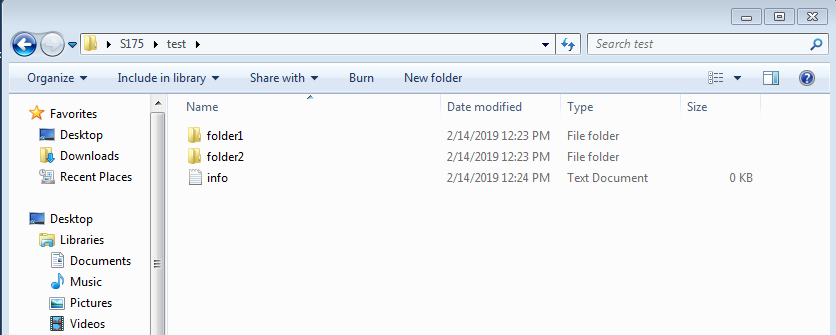
\includegraphics[scale=0.3]{CLI_touch.png}}
\end{figure}
\end{itemize}
\end{frame}

%----------------------------------------------------------
\begin{frame}[fragile]{CLI komandos - cp}
\begin{itemize}
\item \colorbox{listinggray}{\lstinline|cp|}  kopijuoja failą
\begin{lstlisting}
USER@PC MINGW64 ~/Desktop/S175/test
$ cp info.txt info2.txt

USER@PC MINGW64 ~/Desktop/S175/test
$ cp info.txt folder1

USER@PC MINGW64 ~/Desktop/S175/test
$ cp -r folder1 folder2

USER@PC MINGW64 ~/Desktop/S175/test
$ cp -r folder1 /c/Users/USER/Desktop/S175

\end{lstlisting}
\item \colorbox{listinggray}{\lstinline|cp -r folder folder|} arba \colorbox{listinggray}{\lstinline|cp -r folder directory|} -r reiškia, jog kartu kopijuojamas ir folderio turinys
\item Dabar folderyje S175 turime: folder1 ir test

\end{itemize}
\end{frame}

%----------------------------------------------------------
\begin{frame}[fragile]{CLI komandos - rm}
\begin{itemize}
\item \colorbox{listinggray}{\lstinline|rm|} \textit{remove} trina (ne į šiukšliadėžę!!!)
\item \colorbox{listinggray}{\lstinline|rm -r|}  su direktorijos pavadinimu viskam kas direktorijoje
\begin{lstlisting}
USER@PC MINGW64 ~/Desktop/S175/test
$ rm info2.txt

USER@PC MINGW64 ~/Desktop/S175/test
$ rm -r folder2

USER@PC MINGW64 ~/Desktop/S175/test
$ rm -r /c/Users/USER/Desktop/S175/folder1
\end{lstlisting}
\end{itemize}
\end{frame}

%----------------------------------------------------------
\begin{frame}[fragile]{CLI komandos - mw}
\begin{itemize}
\item \colorbox{listinggray}{\lstinline|mw|} perkelia failą (Cut+Paste), arba pervadine failą
\begin{lstlisting}
USER@PC MINGW64 ~/Desktop/S175/test
$ mv info.txt folder1

USER@PC MINGW64 ~/Desktop/S175/test
$ mkdir folderx

USER@PC MINGW64 ~/Desktop/S175/test
$ mv folderx folder2
\end{lstlisting}
\end{itemize}
\end{frame}

%----------------------------------------------------------
\begin{frame}[fragile]{CLI editoriai}
\begin{itemize}
\item Geriausia naudoti \textit{Sublime}
\item \textit{Windows} turi standartinį \textit{Notepad} (tragedija!)
\begin{lstlisting}
USER@PC MINGW64 ~/Desktop/S175/test
$ echo "This is the new text" > info.txt

USER@PC MINGW64 ~/Desktop/S175/test
$ notepad info.txt
\end{lstlisting}
\item Kol neuždarytas Notepad , GitBash "laukimo" būsenoje! tad norint dirbti toliau, pirma reikia uždaryti editorių
\end{itemize}
\end{frame}

%----------------------------------------------------------

\begin{frame}[fragile]{CLI editoriai}
\begin{itemize}
\item GitBash turi \textit{Nano}, bet reikia labai įprasti!
\begin{figure}
\caption{Nano editorius}
\fbox{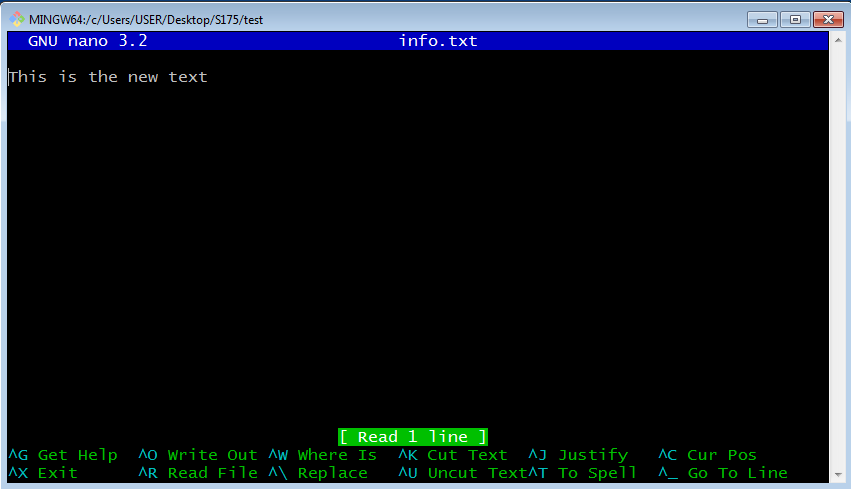
\includegraphics[scale=0.3]{nano_editor_1.png}}
\end{figure}
\end{itemize}
\end{frame}

%----------------------------------------------------------

\begin{frame}[fragile]{CLI editoriai}
\begin{itemize}
\item GitBash turi \textit{Nano}, bet reikia labai įprasti!
\item Atidarome su Nano
\item Įrašome papildomą eilutę
\item Uždarome su Crtl+X, Nano klausia: "Save modified buffer? .."
\item Spaudžiama Y klavišą
\begin{figure}
\caption{Nano editorius}
\fbox{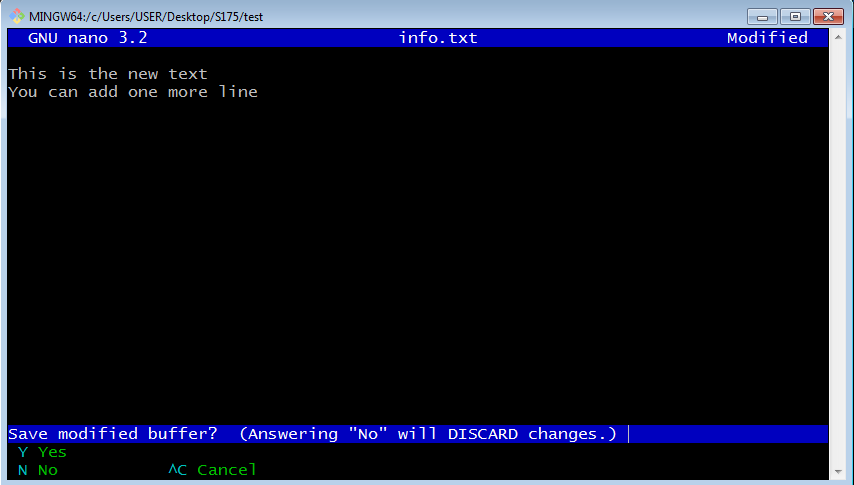
\includegraphics[scale=0.22]{nano_editor_2.png}}
\end{figure}
\end{itemize}
\end{frame}


%----------------------------------------------------------

\begin{frame}[fragile]{CLI editoriai}
\begin{itemize}
\item Nano klausia, ar pavadinimas lieka tas pats?
\item Spaudžiam \textit{Enter} klavišą

\begin{figure}
\caption{Nano editorius}
\fbox{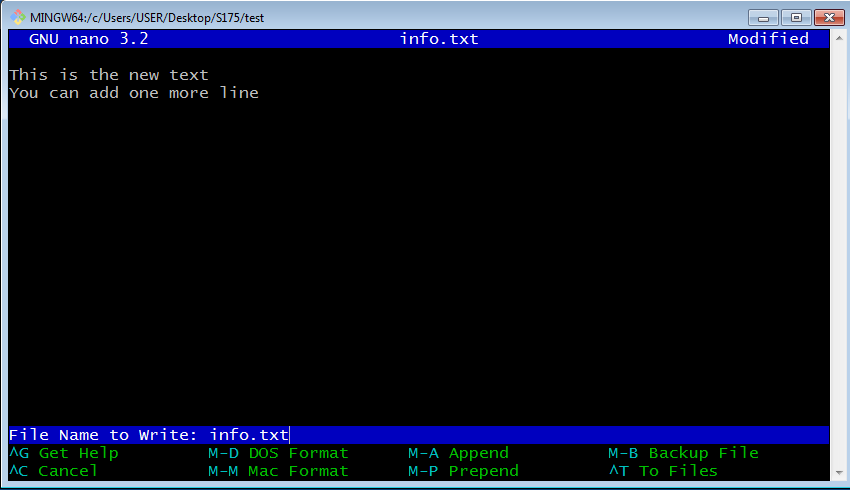
\includegraphics[scale=0.3]{nano_editor_3.png}}
\end{figure}
\end{itemize}
\end{frame}

%----------------------------------------------------------
\begin{frame}[fragile]{Wrap-up}
\begin{itemize}
\item Iki dabar išmokome pagrindinių komandų, kuriomis galime naviguoti sistemoje
\item Taip pat išmokome svarbiausias komandas, kurios ledižia dirbti su failais ir folderiais
\item Tam kad būtų švarus S175/test, belieka tik ištrinti test esančius failus: 
\begin{lstlisting}
USER@PC MINGW64 ~/Desktop/S175/test
$ rm -r folder1
USER@PC MINGW64 ~/Desktop/S175/test
$ rm -r folder2
USER@PC MINGW64 ~/Desktop/S175/test
$ rm info.txt
\end{lstlisting}
\end{itemize}
\end{frame}


%----------------------------------------------------------
\section{Git ir GitHub}
%----------------------------------------------------------

%----------------------------------------------------------
\subsection{Intro}
%----------------------------------------------------------
\begin{frame}{VCS - Version Control System}
\begin{itemize}
\item Kai darbuojatės ir rašote dokumentus, darote juose pakeitimus, dažnai turite 10-20 dokumentų pvz., \colorbox{listinggray}{\lstinline|bakalaurinis.doc|}, \colorbox{listinggray}{\lstinline|bakalaurinis2.doc|}, \colorbox{listinggray}{\lstinline|bakalaurinis2019_01_02.doc|}, \colorbox{listinggray}{\lstinline|bakalaurinis2019_01_02(1).doc|} ir t.t. 
\item dar panašiai tiek pat .xls failų, kiek mažiau skirtingų .ppt failų
\item Galų gale tai veda link chaoso!
\item Todėl labai svarbu, ypač dirbant tu tekstiniais dokumentais (ne Word'iniais), pvz., R skriptais, LaTex failais, turėti vieną failą, bet būti išsisaugojus kartu visas jo ankstesnes formas ir galėti atstatyti ankstesnes jų \textbf{versijas}
\item Bendradarbiaujant su kitais, taip pat svarbu galėti dalintis turimu dokumentu, kodu, leisti kitiems jį keisti ir galų galų integruoti pakeitimus į motininį failą
\end{itemize}
\end{frame}



\begin{frame}{Trumpas įvadas į Git}
\begin{quote}
"Git is a version-control system for tracking changes in computer files and coordinating work on those files among multiple people. It is primarily used for source-code management in software development,but it can be used to keep track of changes in any set of files. As a distributed revision-control system, it is aimed at speed, data integrity, and support for distributed, non-linear workflows"
\end{quote}
\href{https://en.wikipedia.org/wiki/Git}{\textcolor{blue}{https://en.wikipedia.org/wiki/Git}}
\end{frame}
%----------------------------------------------------------
\begin{frame}{Git}
\begin{quote}
"Git is a free and open source distributed version control system designed to handle everything from small to very large projects with speed and efficiency"
\end{quote}
\href{https://git-scm.com/}{\textcolor{blue}{https://git-scm.com/}}
\begin{itemize}
\item Sukurta Linux kurėjo Linus Torvalds
\item Populiariausia VCS
\item Viskas išsaugoma lokaliai
\item GIT naudojamas naudojant CLI, nors Windows yra ir GUI
\item \href{http://git-scm.com/downloads}{\color{blue}Dowload GIT}
\end{itemize}
\end{frame}

%----------------------------------------------------------
\begin{frame}[fragile]{Git pagrdiniai nustatymai}
\begin{itemize}
\item Kiekvienas išsaugojimas bus susietas su išsaugotu "user.name" ir "user.email"
\item Tai reikia padaryti tik vieną kartą (dirbant su savo PC), arba pasikeisti kaskart prisėdus prie svetimo PC
\item Bendradarbiaujant tai padeda atpažinti kas padarė kokius pakeitimus
\item Konfikuruokite Git su savo vardu ir pavarde, bei universiteto email
\end{itemize}
\begin{lstlisting}
$ git config --global user.name "Justas Mundeikis"
$ git config --global user.email justas.mundeikis@evaf.vu.lt
$ git config --global core.pager cat 
$ git config -l
$ git config --global -l
\end{lstlisting}
\end{frame}
%----------------------------------------------------------
\begin{frame}{GitHub}
\begin{quote}
"GitHub  is a web-based hosting service for version control using Git. It is mostly used for computer code. It offers all of the distributed version control and source code management (SCM) functionality of Git as well as adding its own features. It provides access control and several collaboration features such as bug tracking, feature requests, task management, and wikis for every project"
\end{quote}
\href{https://en.wikipedia.org/wiki/GitHub}{\textcolor{blue}{https://en.wikipedia.org/wiki/GitHub}}

\begin{itemize}
\item "push" ir "pull" tarp lokalių ir internetinių repozitorijų
\item suteikia homepage vartotojo repozitorijoms
\item GitHub atlieka back-up funkciją lokalioms repozitorijoms
\item Leidžia bendradarbiauti, dalintis projektais, gerinti kitų kodą ir t.t.
\item GitHub paskyros susikūrimas su VardasPavard (rekomenduotina) ir VU email
\end{itemize}
\end{frame}
%----------------------------------------------------------
\begin{frame}[fragile]{Git}
\begin{itemize}
\item Pirma pasitikriname ar esame .../S175/test ir ar direktorija tuščia
\item tada Inicializuojame git
\begin{lstlisting}
USER@PC MINGW64 ~/Desktop/S175/test
$ pwd
/c/Users/USER/Desktop/S175/test

USER@PC MINGW64 ~/Desktop/S175/test
$ ls -a
./  ../

USER@PC MINGW64 ~/Desktop/S175/test
$ git init
Initialized empty Git repository in C:/Users/USER/Desktop/S175/test/.git/

USER@PC MINGW64 ~/Desktop/S175/test (master)
$ ls -a
./  ../  .git/
\end{lstlisting}
\item direktorijoje sukuriamas nematomas failas .git
\end{itemize}
\end{frame}

%----------------------------------------------------------

\begin{frame}{Git = foto sesija}
\begin{itemize}
\item Git daro "pasirinktos direktorijos nuotraukas" 
\item \textbf{Inicializavimas}, tai tarsi foto kambario pasirinkimas, kuriame gali būti daug "veikėjų"
\item \colorbox{listinggray}{\lstinline|git add failname|} yra tarsi "veikėjo" užvedimas ant foto scenos
\item \colorbox{listinggray}{\lstinline|git commit|} yra pačios nuotraukos darymas
\item Tam kad nuotraukoje nebūtų tam tikrų asmenų galima naudoti sąrašą kuris slepiasi ".gitignore" faile
\end{itemize}
\center
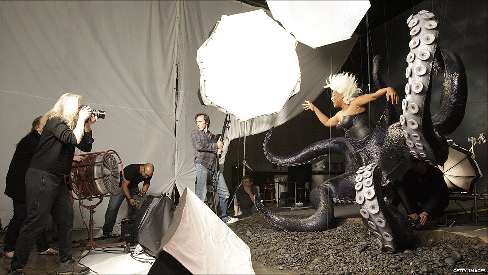
\includegraphics[scale=0.4]{photo_session.png}
\end{frame}

%----------------------------------------------------------
\subsection{Darbas su Git}
%----------------------------------------------------------

\begin{frame}[fragile]{Git}
\begin{itemize}
\item Su komanda touch sukuriame failą readme.txt
\item \colorbox{listinggray}{\lstinline|touch readme.txt|}
\item Su \textit{Sublime} atsidarome readme.txt
\item Įrašome "change1" ir išsaugome failą "Ctrl+S" (uždaryti \textit{Sublime} nereikia)
\end{itemize}
\end{frame}

%----------------------------------------------------------
\begin{frame}{Viskas turėtų atrodyti taip}
\begin{figure}
\caption{Pirmas žingsnis}
\fbox{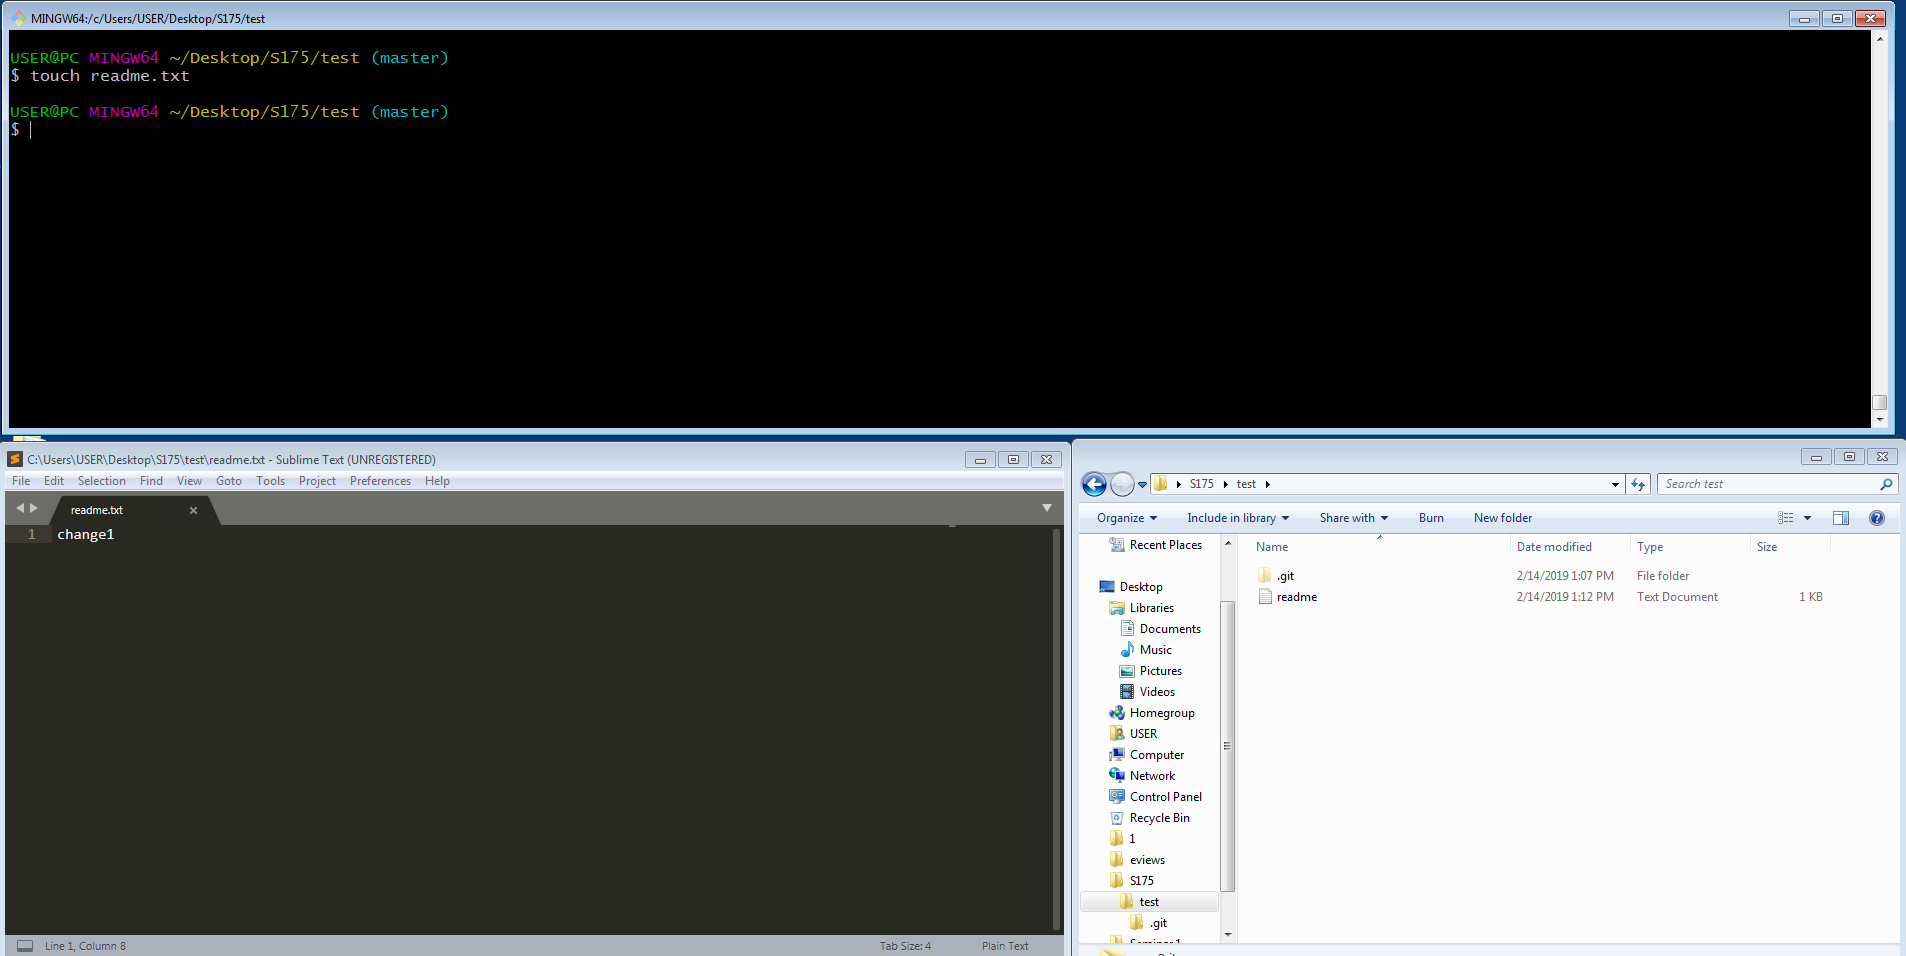
\includegraphics[scale=0.18]{git_flow_1.png}}
\end{figure}
\end{frame}



%----------------------------------------------------------

\begin{frame}[fragile]{Git}
\begin{itemize}
\item Šis failas egzistuoja \textit{repo} (nes jau sekame folderį o to kai parašėme komandą \colorbox{listinggray}{\lstinline|git init|}), tačiau nėra "sekamas"
\begin{lstlisting}
USER@PC MINGW64 ~/Desktop/S175/test (master)
$ git status
On branch master

No commits yet

Untracked files:
  (use "git add <file>..." to include in what will be committed)

        readme.txt

nothing added to commit but untracked files present (use "git add" to track)

\end{lstlisting}
\item Taigi failas readme.txt yra "untracked" kitaip tariant ne ant "scenos"
\end{itemize}
\end{frame}
%----------------------------------------------------------


\begin{frame}[fragile]{Git}
\begin{itemize}
\item su \colorbox{listinggray}{\lstinline|git add readme.txt|} įkeliame readme.txt į \textit{staging area}
\item patikriname statusą:
\begin{lstlisting}
USER@PC MINGW64 ~/Desktop/S175/test (master)
$ git add readme.txt

USER@PC MINGW64 ~/Desktop/S175/test (master)
$ git status
On branch master

No commits yet

Changes to be committed:
  (use "git rm --cached <file>..." to unstage)

        new file:   readme.txt
\end{lstlisting}
\item Taigi failas readme.txt yra \textit{staged} bet dar ne \textit{commited}
\end{itemize}
\end{frame}

%----------------------------------------------------------

\begin{frame}[fragile]{Git}
\begin{itemize}
\item Su Sublime prirašome vieną eilutė "change2", tada Ctrl+S
\item Ką rodo \colorbox{listinggray}{\lstinline|git status|}?
\begin{lstlisting}
USER@PC MINGW64 ~/Desktop/S175/test (master)
$ git status
On branch master

No commits yet

Changes to be committed:
  (use "git rm --cached <file>..." to unstage)

        new file:   readme.txt

Changes not staged for commit:
  (use "git add <file>..." to update what will be committed)
  (use "git checkout -- <file>..." to discard changes in working directory)

        modified:   readme.txt
\end{lstlisting}
\end{itemize}
\end{frame}
%----------------------------------------------------------

\begin{frame}[fragile]{Git}
\begin{itemize}
\item Norint išsaugoti naujausią versiją turime ją pervesti į \textit{staging area}
\item \colorbox{listinggray}{\lstinline|git add readme.txt|}
\begin{lstlisting}
USER@PC MINGW64 ~/Desktop/S175/test (master)
$ git status
On branch master

No commits yet

Changes to be committed:
  (use "git rm --cached <file>..." to unstage)

        new file:   readme.txt
\end{lstlisting}
\item "changes to be commited" reiškia, kad galime fotografuoti
\end{itemize}
\end{frame}

%----------------------------------------------------------
\begin{frame}[fragile]{Git}
\begin{itemize}

\item norint perduoti failą repozitorijai (= fotografuoti)
\begin{lstlisting}
USER@PC MINGW64 ~/Desktop/S175/test (master)
$ git commit -m "sukurtas readme.txt, papildytas change1 ir change2"
[master (root-commit) ca5eddb] sukurtas readme.txt, papildytas change1 ir change2
 1 file changed, 2 insertions(+)
 create mode 100644 readme.txt
 
USER@PC MINGW64 ~/Desktop/S175/test (master)
$ git status
On branch master
nothing to commit, working tree clean
\end{lstlisting}
\item "working tree clean" reiškia, jog esame išsaugoję nuotrauk su visais naujausiais pakeitimais
\end{itemize}
\end{frame}
%----------------------------------------------------------
\begin{frame}{Git commit -m "..."}
\begin{itemize}
\item \colorbox{listinggray}{\lstinline|git commit -m "...."|}
\item -m reiškia "message"
\item Turime apie 72 ženklus, bet galima ir daugiau
\item Aprašas turi būti aiškus, jog būtų prasmingas
\end{itemize}
\begin{figure}
\caption{\href{https://m.xkcd.com/1296/}{\color{blue}{https://m.xkcd.com/1296/}}}
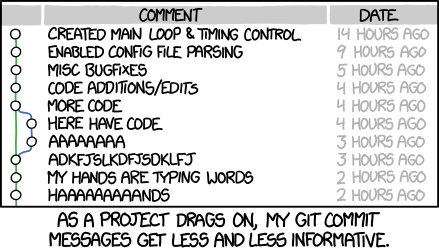
\includegraphics[scale=0.5]{git_commit.png}
\end{figure}
\end{frame}

%----------------------------------------------------------

\begin{frame}[fragile]{Git}
Toliau keičiame naudojamą failą:
\begin{itemize}
\item readme.txt prirašome "change3"
\item \colorbox{listinggray}{\lstinline|git add readme.txt|}
\item \colorbox{listinggray}{\lstinline|git commit -m "pridetas change 3"|}
\item Taigi jau padarėme 2 \textit{commit} (= 2 nuotraukas)
\end{itemize}
\end{frame}

%----------------------------------------------------------
\begin{frame}[fragile]{Git log}
\begin{itemize}
\item Norint žinoti kas, kada ir kaip keitė failą: 
\item \colorbox{listinggray}{\lstinline|git log|}
\begin{lstlisting}
USER@PC MINGW64 ~/Desktop/S175/test (master)
$ git log
commit 030210bb490f45400a706ea69385e8fccc18c65a (HEAD -> master)
Author: Justas Mundeikis <mundeikis@gmx.de>
Date:   Thu Feb 14 13:28:03 2019 -0800

    pridetas change3

commit ca5eddb5fa492038cb3c3d07f483542502bb1e90
Author: Justas Mundeikis <mundeikis@gmx.de>
Date:   Thu Feb 14 13:24:27 2019 -0800

    sukurtas readme.txt, papildytas change1 ir change2

\end{lstlisting}
\end{itemize}
\end{frame}

%----------------------------------------------------------
\begin{frame}[fragile]{Git log --oneline}
\begin{itemize}
\item Norint žinoti kas, kada ir kaip keitė failą, bet gauti mažiau info
\item \colorbox{listinggray}{\lstinline|git log --oneline|}
\begin{lstlisting}
USER@PC MINGW64 ~/Desktop/S175/test (master)
$ git log --oneline
030210b (HEAD -> master) pridetas change3
ca5eddb sukurtas readme.txt, papildytas change1 ir change2
\end{lstlisting}
\end{itemize}
\end{frame}

%----------------------------------------------------------

\begin{frame}[fragile]{Git}
\begin{itemize}
\item Dabar sukursime naują failą \textit{basic.R} ir \textit{readme.txt} pridėsime change4
\item \colorbox{listinggray}{\lstinline|touch basic.R|}
\item readme.txt įrašome "change4", išsaugome
\item \colorbox{listinggray}{\lstinline|git status|} parodo, jog pakeistas \textit{readme.txt} failas, ir untracked \textit{basic.R} failas
\item su komanda \colorbox{listinggray}{\lstinline|git add .|} staginame visus failus
\item galimi kiti variantai : \colorbox{listinggray}{\lstinline|git add -A|},\colorbox{listinggray}{\lstinline|git add -u|} (pastarasis naudojamas tik update'inti jau sekamus failus)
\item tada \colorbox{listinggray}{\lstinline|git commit -m "pridedamas change4 ir sukuriamas failas basic.R"|}
\end{itemize}
\end{frame}
%----------------------------------------------------------

\begin{frame}[fragile]{Git}
\begin{itemize}
\item Kartais yra tam tikri failai, kurių nenorime sekti (pvz duomenys, nereikalingi LaTex failai ir t.t.)
\item Sukuriame duomenų failą
\item \colorbox{listinggray}{\lstinline|touch data.csv|} 
\item \colorbox{listinggray}{\lstinline|git status|} parodo failą kaip \textit{untracked}
\item todėl sukuriame failą \colorbox{listinggray}{\lstinline|touch .gitignore|}, kuriame galima surašyti failų pavadinimus, arba failų tipą/galūnes, kurių nenorime trackinti
\item \textit{Sublime} įrašome:  \colorbox{listinggray}{\lstinline|*.csv|} 
\item * reiškia bet kokį pavadinimą, po kurio seka taškas ir csv, alternatyviai galima specifikuoti konkretų failą "data.csv"
\item "git status" neberodo failo "data.csv" bet rodo ".gitignore", todėl staginame ir commitiname pakeitimus
\item \colorbox{listinggray}{\lstinline|git add .|} ir  \colorbox{listinggray}{\lstinline|git commit -m "sukurtas gitignore sarasas"|}  
\end{itemize}
\end{frame}

%----------------------------------------------------------
\subsection{Git branch}
%----------------------------------------------------------

\begin{frame}[fragile]{Git branch'inimas}
\begin{itemize}
\item Bazinis scenarijus:
\begin{itemize}
\item A kuria projektą, B nori prisidėti, tačiau ir A dirba tuo pat metu...
\item B atsiskelia atšaką (branch'ina) A projektą, padaro savo pakeitimus ir pateikia A juos sujungti
\item A peržiūri pakeitimus, priima/atmeta
\end{itemize}
\end{itemize}
\end{frame}

\begin{frame}[fragile]{Git branch'inimas}
\begin{itemize}

\item \colorbox{listinggray}{\lstinline|git branch NewBranch|}  sukuria naują atšaką pavadinimu \textit{NewBranch}
\item \colorbox{listinggray}{\lstinline|git checkout NewBranch|} išmeta iš "master" į \textit{NewBranch}
\item \colorbox{listinggray}{\lstinline|git checkout master|} visada sugrąžina atgal į \textit{master} šaką

\begin{lstlisting}
USER@PC MINGW64 ~/Desktop/s175/test (master)
$ git branch NewBranch

USER@PC MINGW64 ~/Desktop/s175/test (master)
$ git checkout NewBranch
Switched to branch 'NewBranch'
\end{lstlisting}

\item dabar visi pakeitimai vyks tik šioje atšakoje ir nepaveiks \textit{master} šakos
\end{itemize}
\end{frame}
%----------------------------------------------------------

\begin{frame}{Darbas Git atšakoje}
Tarkime dabar asmuo B darbuojasi NewBranch atšakoje tobulindamas projektą
\begin{itemize}
\item \colorbox{listinggray}{\lstinline|touch advanced.R|}
\item \colorbox{listinggray}{\lstinline|notepad readme.txt|} įrašome papildomą eilutę "change5", tada Crtl+S
\item staginam ir commitinam pakeitimus:
\begin{itemize}
\item \colorbox{listinggray}{\lstinline|git add .|}
\item \colorbox{listinggray}{\lstinline|git commit -m "sukuriamas advanced.R ir pridedmas change5"|}
\end{itemize}
\item sugrįžtame į master atšaką su \colorbox{listinggray}{\lstinline|git checkout master|}
\item Rezultatas: trūksta \textit{advanced.R} failo, \textit{readme.txt} turi tik 4 įrašus!
\item Norint sujungti naują atšaką į \textit{master} \colorbox{listinggray}{\lstinline|git merge NewBranch|}
\end{itemize}
\end{frame}

%----------------------------------------------------------
\begin{frame}[fragile]{Git merge}
\begin{itemize}
\item \colorbox{listinggray}{\lstinline|git merge NewBranch|}
\item \colorbox{listinggray}{\lstinline|git log --oneline|}

\begin{lstlisting}
USER@PC MINGW64 ~/Desktop/S175/test (master)
$ git merge NewBranch
Updating b8940f7..407d27c
Fast-forward
 advanced.R | 0
 readme.txt | 3 ++-
 2 files changed, 2 insertions(+), 1 deletion(-)
 create mode 100644 advanced.R
 
USER@PC MINGW64 ~/Desktop/S175/test (master)
$ git log --oneline
407d27c (HEAD -> master, NewBranch) sukuriamas advanced.R ir pridedmas change5
b8940f7 sukurtas gitignore sarasas
ebff561 pridedamas change4 ir sukuriamas failas basic.R
030210b pridetas change3
ca5eddb sukurtas readme.txt, papildytas change1 ir change2

\end{lstlisting}
\end{itemize}
\end{frame}




%----------------------------------------------------------
\begin{frame}[fragile]{Merge problemos}
\begin{itemize}
\item Kartais nutinka taip, kad atšakoje esantys failai ne visai atitinka su master šakoje esančiais failais, todėl juos jungiant kyla problemų, kurias reikia pašalinti "ranka"
\item \textit{master} atšakoje \textit{readme.txt} sukuriame eilutę "change5",Ctrl+S, stage'inam ir commit'iname 
\item Nueiname į atšaką \textit{NewBranch} ir ten esančiame \textit{readme.txt} sukuriame "change7", stage'inam ir commit'iname 
\item grįžtame į \textit{master} atšaką \colorbox{listinggray}{\lstinline|git chekckout master|}
\item ir bandome sujungti \colorbox{listinggray}{\lstinline|git merge NewBranch|}
\end{itemize}
\end{frame}

%----------------------------------------------------------

\begin{frame}[fragile]{Merge problemos}
\begin{itemize}
\begin{lstlisting}
USER@PC MINGW64 ~/Desktop/S175/test (master)
$ git merge NewBranch
Auto-merging readme.txt
CONFLICT (content): Merge conflict in readme.txt
Automatic merge failed; fix conflicts and then commit the result.
\end{lstlisting}

\item Git negalėjo automatiškai sutvarkyti failų (kaip pirmą kartą), nes dabar toje pačioje readme.txt failo vietoje vienur yra "change6" kitur "change7". Todėl atsidarome readme.txt failą ir tvarkome patys
\end{itemize}
\end{frame}
%----------------------------------------------------------

\begin{frame}[fragile]{Konfliktinio failo tvarkymas}
\begin{itemize}
\item Atsidarius readme.txt matome
\begin{figure}
\caption{Merge problema}
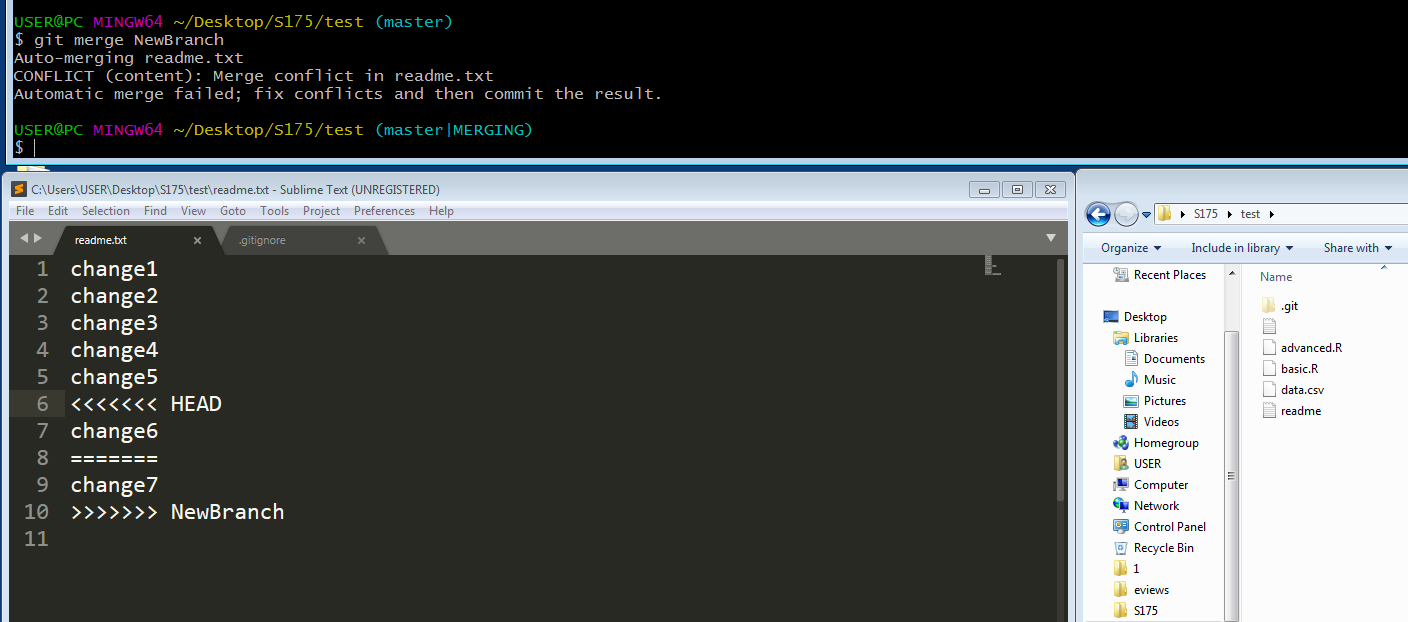
\includegraphics[scale=0.2]{git_flow_2}
\end{figure}

\item $<<<<<HEAD$ yra tai kas yra aktyvioje atšakoje
\item $>>>>NewBranch$ yra kas ateina iš sujungiamos atšakos
\item atskirta ======
\end{itemize}
\end{frame}

%----------------------------------------------------------

\begin{frame}[fragile]{Konfliktinio failo tvarkymas}
\begin{itemize}
\item Sutvarkome failą, taip kaip norime
\begin{lstlisting}
change1
change2
change3
change4
change5
change6
change7
\end{lstlisting}
\item Išsaugome pakeitimus Ctrl+S, tada
\item \colorbox{listinggray}{\lstinline|git commit -a -m "sujungtas failas is NewBranch bei pasalintas konfliktas|}
\item  \colorbox{listinggray}{\lstinline|git commit -a -m "..."|} galima naudoti, jeigu nėra sukurtų naujų failų
\item Yra papildomų įrankių, kurie padeda atlikti merge'inimo darbus, nes dažniausiai konfliktų visada bus
\end{itemize}
\end{frame}

%----------------------------------------------------------

\begin{frame}[fragile]{Git atsatatymas 1}
\begin{itemize}
\item Imituojame, jog dirbome ir sukūrėme gerą failą ir paskui jį papildėme blogu:
\begin{lstlisting}
USER@PC MINGW64 ~/Desktop/S175/test (master)
$ echo "sukuriamas geras failas" > svarbus.txt
$ git add .
$ git commit -m "sukurtas svarbus.txt"
$ echo "12 nakties pridirbau nesamoniu" >> svarbus.txt
$ git commit -a -m "pridirbta nesamone"
$ git log --oneline
78839b7 (HEAD -> master) pridirbta nesamone
9547650 sukurtas svarbus.txt
2a982aa merge klaida panaikinta, change6 ir change7
26e6ae0 (NewBranch) sukurtas change7
8562e69 sukurtas change6
407d27c sukuriamas advanced.R ir pridedmas change5
b8940f7 sukurtas gitignore sarasas
ebff561 pridedamas change4 ir sukuriamas failas basic.R
030210b pridetas change3
ca5eddb sukurtas readme.txt, papildytas change1 ir change2
\end{lstlisting}
\end{itemize}
\end{frame}

%----------------------------------------------------------


\begin{frame}[fragile]{Git atsatatymas}
\begin{itemize}
\item Norint susigrąžinti failą į praėjusią "gerą" būseną, reikia susirasti "blogo" commit hashą  mano atveju (žr. viršuje) 78839b7
\item \colorbox{listinggray}{\lstinline|git log --oneline|}
\item komanda \colorbox{listinggray}{\lstinline|git revert HASH|} atstato pasirinktą versiją, versijos su "12 nakties..." nebėra!
\item komanda \colorbox{listinggray}{\lstinline|git revert 78839b7|}
\item po įvedimo atsiranda \textit{message} langas (atitinka -m "...."), nes revert'inimas yra naujas commit
\end{itemize}
\end{frame}


%----------------------------------------------------------

\begin{frame}[fragile]{Git atstatymas}
\begin{figure}
\caption{Revert atidaro messge su nano}
\fbox{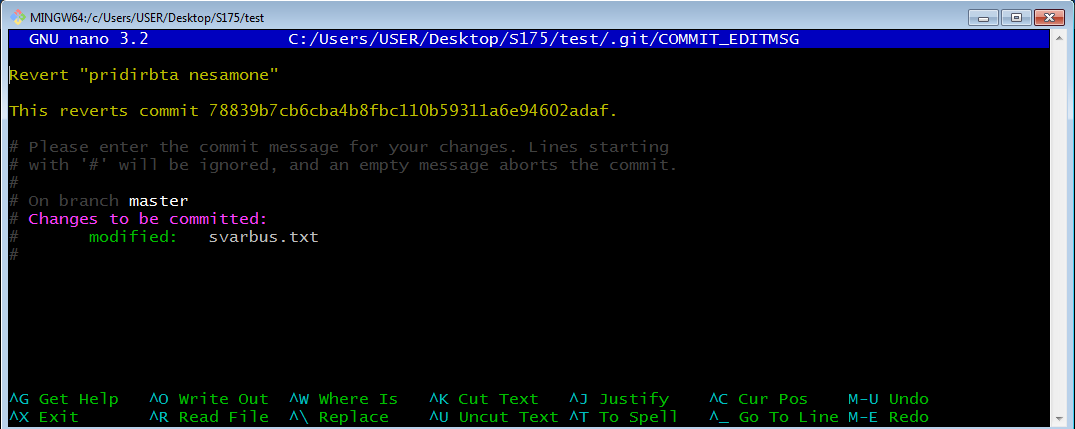
\includegraphics[scale=0.3]{git_revert_1.png}}
\end{figure}
\begin{itemize}
\item Spaudžiame Crtl+X ir vėl atsiduriame normaliame Git
\end{itemize}
\end{frame}

%----------------------------------------------------------

\begin{frame}[fragile]{Git atstatymas}
\begin{itemize}
\item Tik jau blogojo įrašo \textit{Sublime} neberodo
\end{itemize}
\begin{figure}
\caption{Po revert}
\fbox{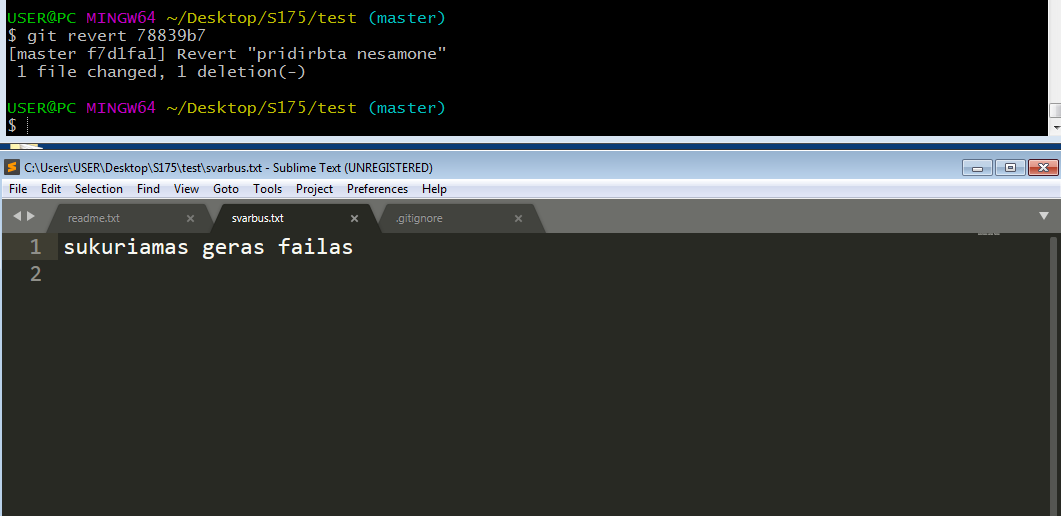
\includegraphics[scale=0.25]{git_revert_2.png}}
\end{figure}
Spaudžiame Crtl+X ir vėl atsiduriame normaliame Git
\end{frame}


%----------------------------------------------------------

\begin{frame}[fragile]{Git reset}
\begin{itemize}
\item Atsargiai! 
\item Tarkime jus labai daug darbavotės, turite n commit padarę ir supratote, kad pirmas commit buvo geras, o po to viskas ne.
\item \colorbox{listinggray}{\lstinline|git revert HASH|} palieka buvusias versijas, bet šiuo atveju, jos nebereikalingos
\item \colorbox{listinggray}{\lstinline|git reset --hard HASH|} komanda padaro hard-reset, t.y. resetina į pasirinktą commitą, tačiau ištrina viską, kas buvo daryta po to! 
\item revert'inti \colorbox{listinggray}{\lstinline|git reset --hard HASH|} neįmanoma, priešingai nei paties revert.
\item Taigi geriau su hard-reset nesižaist :D
\end{itemize}
\end{frame}

%----------------------------------------------------------

\begin{frame}[fragile]{Git branch ištrynimas}
\begin{itemize}
\item Mums nebereikia NewBranch atšakos
\item Kiek šakų turime patikrinti galima su \colorbox{listinggray}{\lstinline|git branch|}. * parodo kur esame
\item Nereikalingą šaką ištrinti galime su komanda \colorbox{listinggray}{\lstinline|git branch -d Newbranch|} -d = delete
\begin{lstlisting}
USER@PC MINGW64 ~/Desktop/S175/test (master)
$ git branch
  NewBranch
* master

USER@PC MINGW64 ~/Desktop/S175/test (master)
$ git branch -d NewBranch
Deleted branch NewBranch (was 26e6ae0).

USER@PC MINGW64 ~/Desktop/S175/test (master)
$ git branch
* master
\end{lstlisting}
\end{itemize}
\end{frame}

%----------------------------------------------------------

\begin{frame}{Git remote}
\begin{itemize}
\item norint žinoti, ar lokali repozitorija yra susieta su nuotoline repozitorija (pvz Github, Bitbucket ar pan)
\item \colorbox{listinggray}{\lstinline|git remote|}
\item Jeigu komanda neišmeta jokios informacijos, reiškia lokali \textit{repo} nesusieta su nuotoline \textit{repo}
\end{itemize}
\end{frame}

%----------------------------------------------------------

\begin{frame}{Git remote}
\begin{itemize}
\item Nueiname kiekvienas į savo GitHub ir ten susikuriame repo:
\begin{itemize}
\item pavadinimas: test
\item Description paliekam tučią
\item NE inicializuojame su README!!!!
\end{itemize}
\item keliaujame į savo "test" direktoriją
\item \colorbox{listinggray}{\lstinline|git remote add origin HTPPS|}
\item \colorbox{listinggray}{\lstinline|git push - u origin master|}
\end{itemize}
\end{frame}

\begin{frame}{Git remote}
\begin{figure}
\caption{Nuotolinės repo kūrimas @GitHub: spaudžiam and + ir tada "New repository"}
\fbox{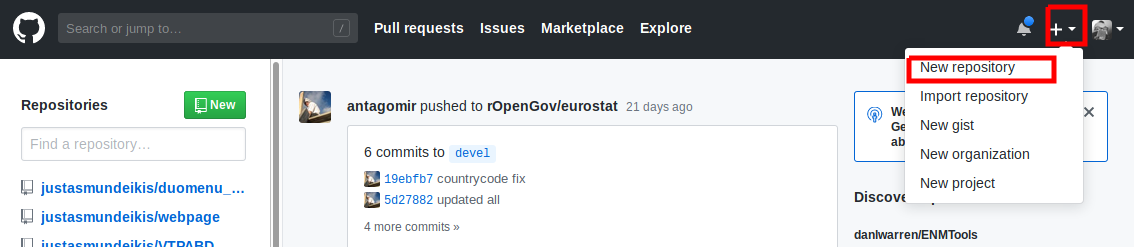
\includegraphics[scale=0.3]{git_remote_1}}
\end{figure}
\end{frame}

\begin{frame}{Git remote}
\begin{figure}
\caption{Nuotolinės repo kūrimas @GitHub: pavadinimas :test, Initialize paliekam tuščią ir spaudžiam "Creat repository"}
\fbox{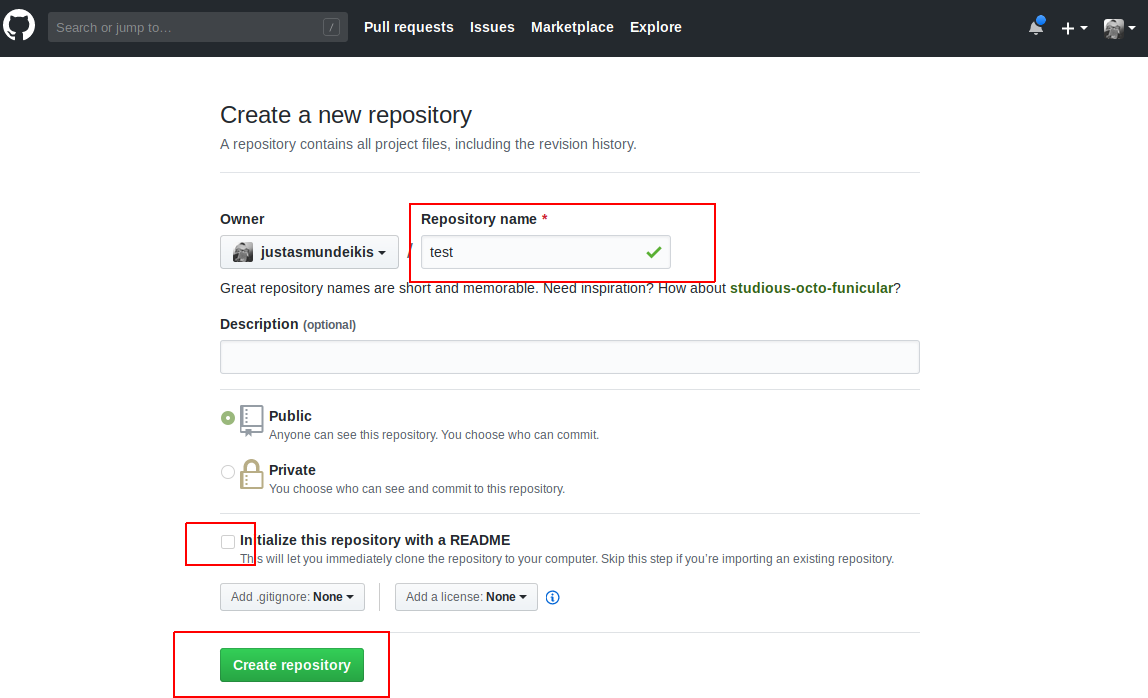
\includegraphics[scale=0.23]{git_remote_2}}
\end{figure}
\end{frame}


\begin{frame}{Git remote}
\begin{figure}
\caption{Nuotolinės repo kūrimas @GitHub: šis langas pasako, kaip lokalinę repo sujungti su nuotoline...}
\fbox{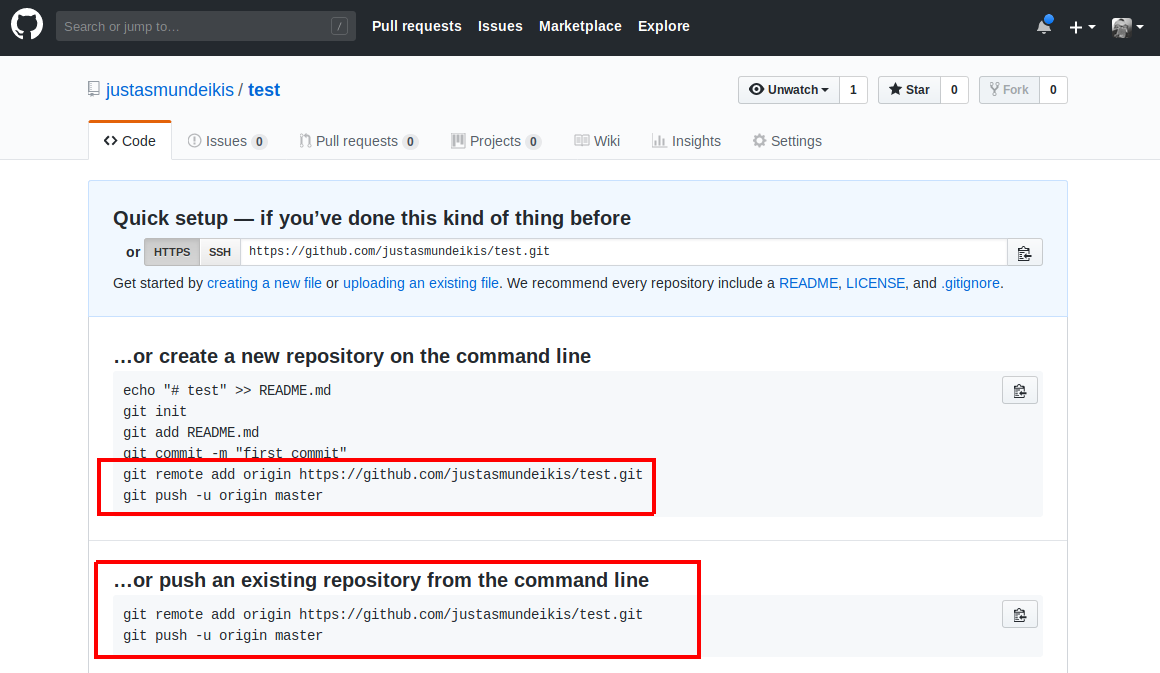
\includegraphics[scale=0.2]{git_remote_3}}
\end{figure}
\end{frame}

%----------------------------------------------------------

\begin{frame}[fragile]{Git remote}
\begin{itemize}
\item po \colorbox{listinggray}{\lstinline|git push|} reikės įrašyti savo email (GitHub) ir pop-up lange savo passwordą
\item po \colorbox{listinggray}{\lstinline|git remote -v|} parodo daugiau info apie remote repo
\begin{lstlisting}
$ git remote add origin https://github.com/justasmundeikis/test.git
$ git remote -v
origin  https://github.com/justasmundeikis/test.git (fetch)
origin  https://github.com/justasmundeikis/test.git (push)
$ git push origin master
Username for 'https://github.com': vardas.pavarde@stud.vu.lt
Enumerating objects: 32, done.
Counting objects: 100% (32/32), done.
Delta compression using up to 2 threads
Compressing objects: 100% (21/21), done.
Writing objects: 100% (32/32), 2.55 KiB | 55.00 KiB/s, done.
Total 32 (delta 8), reused 0 (delta 0)
remote: Resolving deltas: 100% (8/8), done.
To https://github.com/justasmundeikis/test.git
 * [new branch]      master -> master
\end{lstlisting}
\end{itemize}
\end{frame}


%----------------------------------------------------------

\begin{frame}[fragile]{Git remote}
\begin{figure}
\caption{Su F5 refresh'inus GitHub puslapį matome, jog vietinio folderio turinys visas perkeltas į GitHub}
\fbox{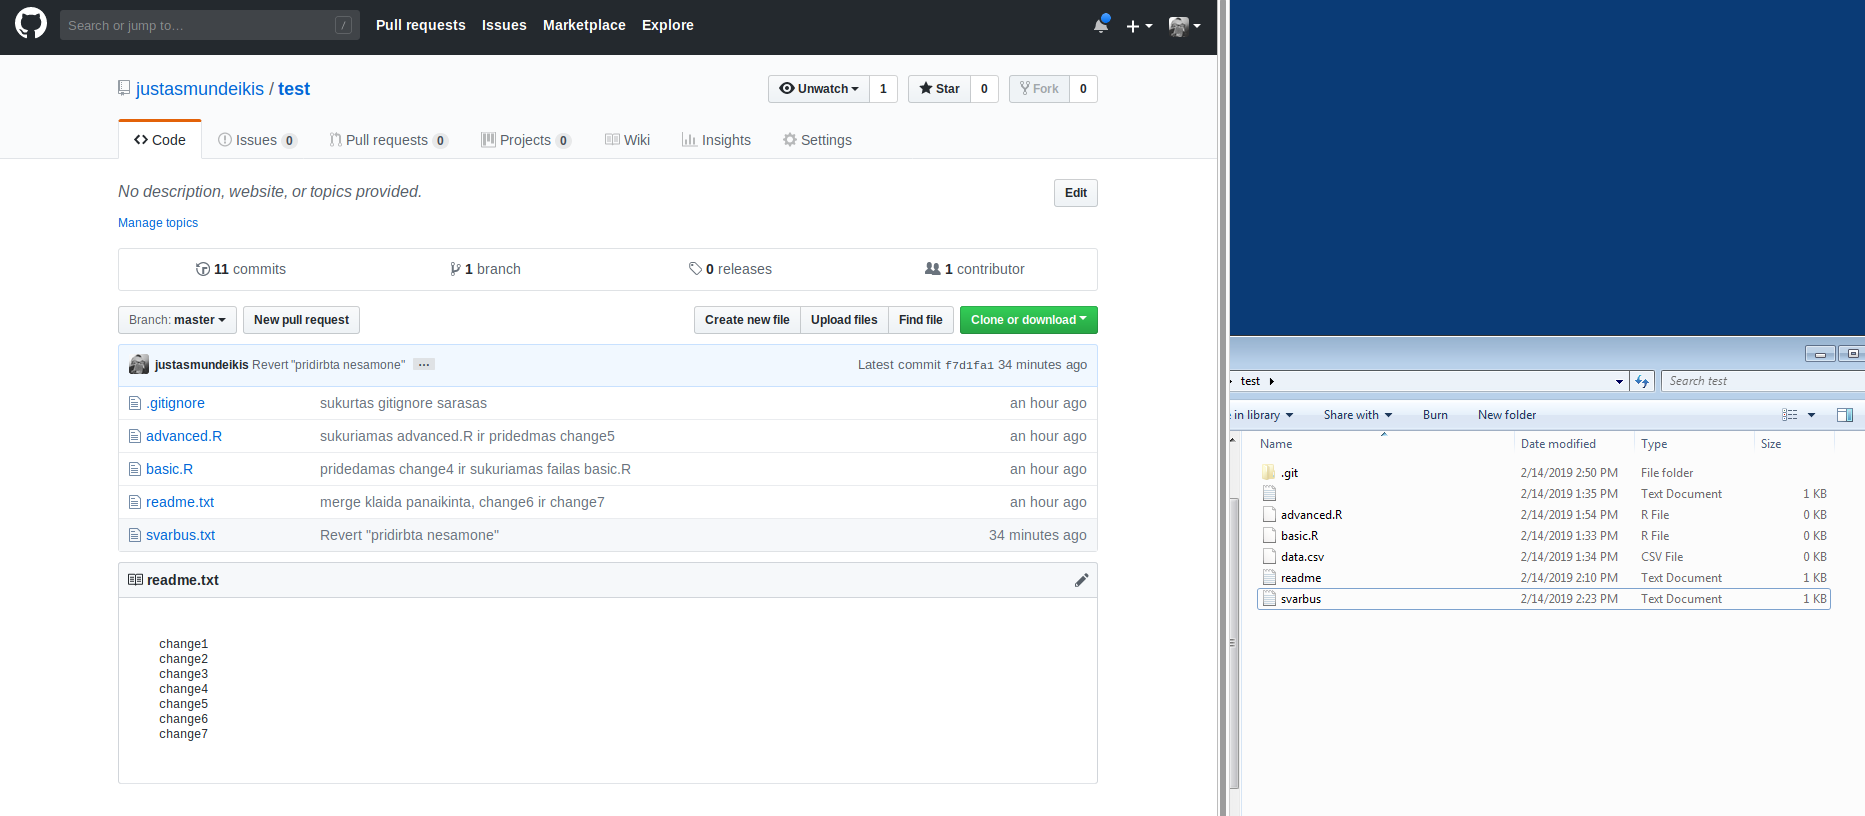
\includegraphics[scale=0.18]{git_remote_4}}
\end{figure}
\end{frame}


%----------------------------------------------------------
\begin{frame}
\begin{itemize}
\item Sveikinu su pirmu išsiuntimu savo darbo į internetą
\item Suprantama, galima pirma sukurti repo @GitHub ir tada sukurtą repo klonuoti į savo PC tai, sekantis žingsnis
\item Klonuoti galima ir "svetimas" repo
\end{itemize}
\end{frame}

%----------------------------------------------------------

\begin{frame}{Git repo klonavimas}
\begin{itemize}
\item Kiekvienas į savo GitHub paskyroje susikuriame repo:
\begin{itemize}
\item Pavadinimas: test2
\item Description paliekam tuščią
\item inicializuojame su Readme.md
\end{itemize}
\begin{figure}
\caption{Sukuriama nauja repo "test2"}
\fbox{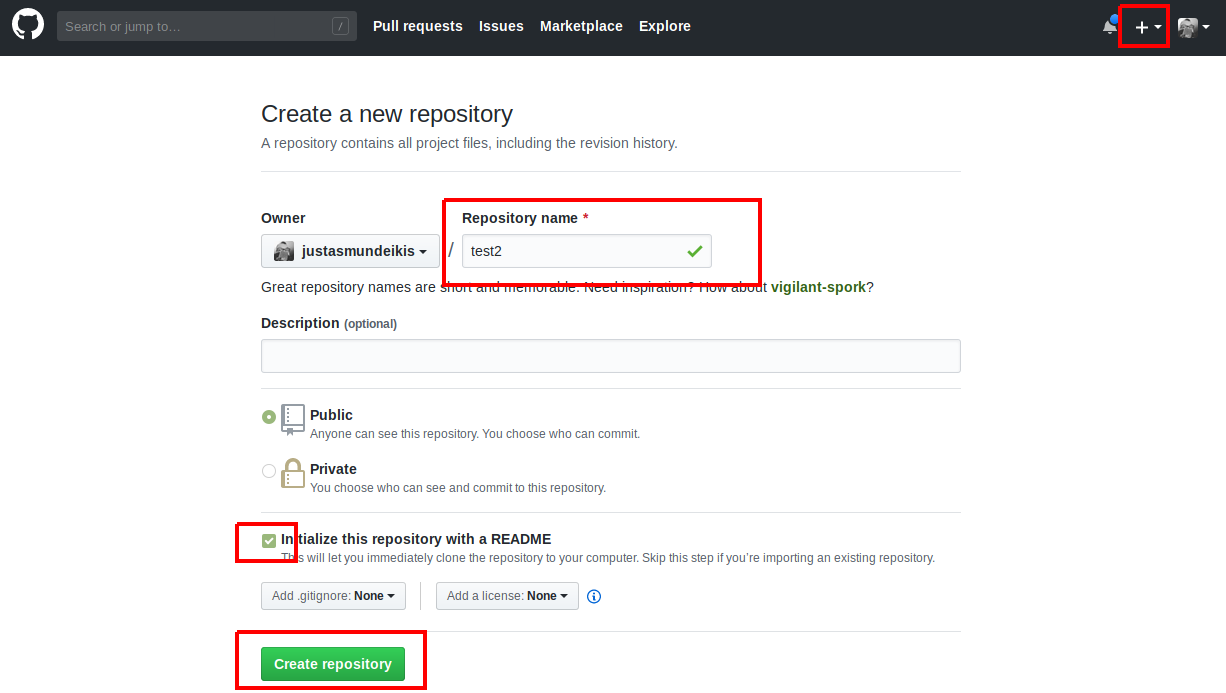
\includegraphics[scale=0.18]{git_remote_5.png}}
\end{figure}
\end{itemize}
\end{frame}

%----------------------------------------------------------

\begin{frame}{Git repo klonavimas}
\begin{itemize}
\item GitHub nusikopijuojame sukurtos repo HTTPS adresą
\begin{figure}
\caption{Nukopijuojamas repo HTTPS}
\fbox{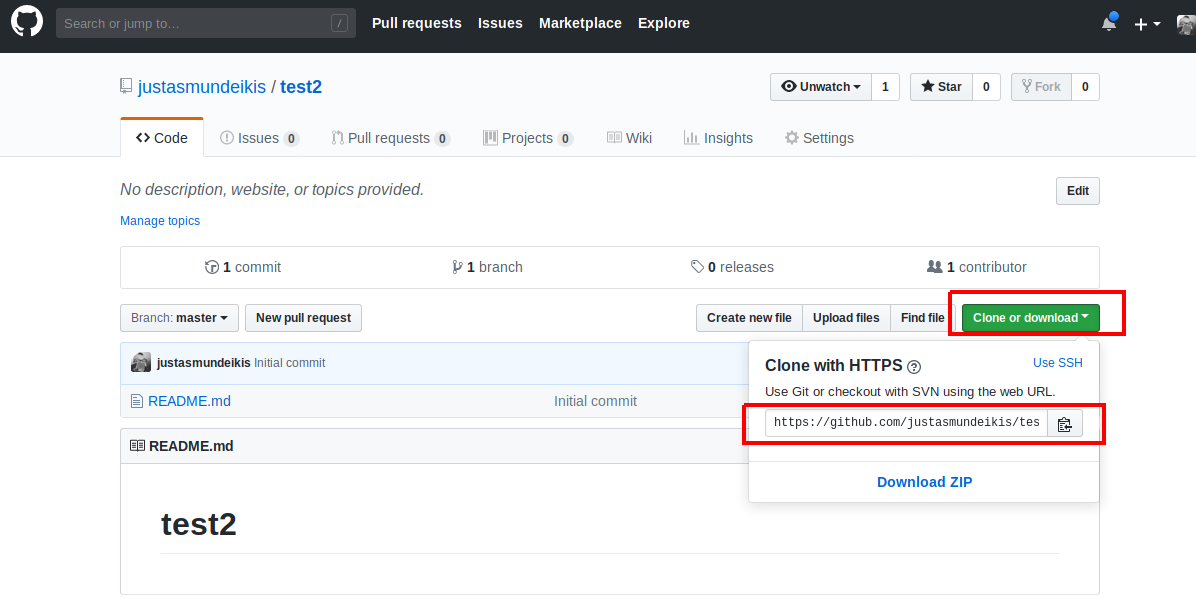
\includegraphics[scale=0.2]{git_remote_6.png}}
\end{figure}
\end{itemize}
\end{frame}

%----------------------------------------------------------

\begin{frame}[fragile]{Git repo klonavimas}
\begin{itemize}
\item Git Bash lange pakylame viena direktorija aukščiau, įsitikiname ar esame S175 folderyje ir klonuojame nusikopijuotą adresą:
\begin{lstlisting}
USER@PC MINGW64 ~/Desktop/S175/test (master)
$ cd ..

USER@PC MINGW64 ~/Desktop/S175
$ pwd
/c/Users/USER/Desktop/S175

USER@PC MINGW64 ~/Desktop/S175
$ git clone https://github.com/justasmundeikis/test2.git
Cloning into 'test2'...
remote: Enumerating objects: 3, done.
remote: Counting objects: 100% (3/3), done.
remote: Total 3 (delta 0), reused 0 (delta 0), pack-reused 0
Unpacking objects: 100% (3/3), done.
\end{lstlisting}
\end{itemize}
\end{frame}


%----------------------------------------------------------

\begin{frame}[fragile]{Git repo klonavimas}
\begin{itemize}
\item Klonuotoje repo, sukursime failą, ir jį nusiųsime atgal į GitHub"
\item pareikalavus įrašome github username ir userpassword
\item GitHub atnaujiname (F5) ir voila, failas info.txt yra remote repozitorijoje (\colorbox{listinggray}{\lstinline|&&|}) apjungia dvi komandas vienoje eilutėje
\begin{lstlisting}
USER@PC MINGW64 ~/Desktop/S175
$ pwd
/c/Users/USER/Desktop/S175

USER@PC MINGW64 ~/Desktop/S175
$ cd test2

USER@PC MINGW64 ~/Desktop/S175
$ echo "test2 klonavimas ir siuntimas i Github" >about.txt

USER@PC MINGW64 ~/Desktop/S175
$ git add . && git commit -m "sukurtas about.txt"

USER@PC MINGW64 ~/Desktop/S175
$ git push
\end{lstlisting}

\end{itemize}
\end{frame}

%----------------------------------------------------------

\begin{frame}[fragile]{Git repo klonavimas}
\begin{itemize}
\item Sveikinu, sukūrėte GitHub repo
\item Ją klovanote
\item Pakeitėte vietinėje repo failus
\item Ir juos pushinote į Github!
\item Atnaujine Github, pamatysite savo naujai sukurtą failą!
\end{itemize}
\end{frame}
%----------------------------------------------------------

\begin{frame}{Git repo klonavimas}
\begin{itemize}
\item Dabar klonuokite dar vieną folderį:
\item Tačiau pirma įsitikinite, ar esate S175 folderyje, jeigu ne, pereikite (žr sekanti skaidrė)
\item \colorbox{listinggray}{\lstinline|git clone https://github.com/justasmundeikis/duomenu_analizes_ivadas.git|}
\item Sveikinu, atsisiuntėte mano paskaitų medžiagą
\item Norint žinoti ar nėra jokių paskaitos medžiagų atnaujinimo, galima nuėjus į patį folderį įrašyti komandą
\item \colorbox{listinggray}{\lstinline|git pull|} 
\end{itemize}
\end{frame}


\begin{frame}[fragile]{Git repo klonavimas}
\begin{lstlisting}
USER@PC MINGW64 ~/Desktop/S175
$ pwd
/c/Users/USER/Desktop/S175

$ git clone https://github.com/justasmundeikis/duomenu_analizes_ivadas.git
Cloning into 'duomenu_analizes_ivadas'...

USER@PC MINGW64 ~/Desktop/S175
$ ls
duomenu_analizes_ivadas/  test/  test2/

USER@PC MINGW64 ~/Desktop/S175
$ cd duomenu_analizes_ivadas/

USER@PC MINGW64 ~/Desktop/S175/duomenu_analizes_ivadas (master)
$ git pull
Already up to date.
\end{lstlisting}

\end{frame}



%----------------------------------------------------------
\subsection{Markdown sintaksė}
%----------------------------------------------------------
\begin{frame}[fragile]{Markdown sintaksė}
\begin{itemize}
\item GitHub sukuriant repo, ją galima inicijuoti su readme.md
\item .md reiškia, jog tai yra markdown formatas
\item Markdown is a lightweight markup language with plain text formatting syntax. Its design allows it to be converted to many output formats, but the original tool by the same name only supports HTML. Markdown is often used to format readme files, for writing messages in online discussion forums, and to create rich text using a plain text editor. (\href{https://en.wikipedia.org/wiki/Markdown}{\textcolor{blue}{https://en.wikipedia.org/wiki/Markdown}})
\item Labai trumpa pagalba dėl formatavimo: \href{https://commonmark.org/help/}{\textcolor{blue}{https://commonmark.org/help/}}
\item Vėliau mes susipažinsime su RMarkdown
\end{itemize}
\end{frame}

%----------------------------------------------------------
\section{Google Scholar}
%----------------------------------------------------------
\begin{frame}{Google Scholar}
\begin{itemize}
\item Viskas prasideda nuo daug skaitymo, tarkime aptinkate  \href{https://www.economist.com/graphic-detail/2019/02/13/a-no-deal-brexit-would-affect-more-than-just-british-trade-with-the-eu}{\color{blue}{"The Economist"}} straipsnį apie \textit{"Brexit"}
\item Nusprendžiate kad esė tema galėtų būti "Kaip Brexit paveiks Lietuvos ekonomiką"
\item Dabar reikia eiti ieškoti moklsinių straipsnių, geriausiai tam tinka...
\item \href{https://scholar.google.lt/}{\color{blue}{https://scholar.google.lt/}}
\item Funkcijos
\begin{itemize}
\item Laikotarpis
\item Kurti įspėjjimą
\item citavimas
\item Cituoja
\item Visos versijos
\item AND OR 
\item Išplėstinė paieška
\end{itemize}
\item Dabar galime kartoti temos pavadinimo / klausimo epiciklą

\end{itemize}
\end{frame}
%----------------------------------------------------------
\begin{frame}{Literatūra}
\begin{itemize}
\item Apie duomenų analizė R.D. Peng \& E.Matsui: "The Art of Data Science" 1-3 skyriai
\item CLI patarčiau šią mokamąją medžiagą: \href{https://www.learnenough.com/command-line-tutorial/basics}{\color{blue}{Learn Enough Command Line to Be Dangerous}}
\item Git patarčiau šią mokamąją medžiagą: \href{https://www.learnenough.com/git-tutorial/getting_started}{\color{blue}{Learn Enough Git to Be Dangerous}}
\item Youtube: ieškant "Git Basics"
\end{itemize}
\end{frame}

\begin{frame} {Namų darbai}
\begin{itemize}
\item Namuose instaliuoti visas reikalingas programas (Git, Sublime)
\item Pakartoti skaidrėse praeitus žingsnius
\item Išspręsti Seminar 1 užduotis
\item VU VMA įkelti savo Seminar 1 dokumento prašomas nuorodas
\item Reguliariai pasitikrinti, ar nėra VMA įkeltų straipnsių skaitumui, jeigu yra, perskaityti, nes apie savaitinius skaitinius gali būti klausiama teste!!!

\end{itemize}
\end{frame}

\end{document}